\documentclass[10pt]{ltjsarticle}
\usepackage{tcolorbox}
\usepackage{float}
\usepackage{pdfpages}
\include{graphicx}
\usepackage{subcaption}  % subcaption パッケージの読み込み
\usepackage{float}       % [H] オプションを使用するため
% \usepackage{caption}
% \usepackage{multirow}
% \usepackage{hhline}
% \usepackage{ascmac}
% \usepackage{mathrsfs}
% \usepackage{amsmath}
% \usepackage{amssymb}
\usepackage{url}

% ? Tikz config =========================
% \usepackage{tikz}
% \usetikzlibrary{shapes.geometric}
% \usetikzlibrary {shapes.misc}
% \usetikzlibrary{positioning}
% \usetikzlibrary{calc}
% ? =====================================

% ? Listing config ======================
% \usepackage{listings,jvlisting}
% \lstset{
%   basicstyle={\ttfamily},
%   identifierstyle={\small},
%   commentstyle={\smallitshape},
%   keywordstyle={\small\bfseries},
%   ndkeywordstyle={\small},
%   stringstyle={\small\ttfamily},
%   basewidth=0.5em,
%   frame=none,
%   breaklines=true,
%   xleftmargin=0pt,
%   xrightmargin=0pt,
%   framexleftmargin=22pt,
%   columns=fixed,
%   numbers=left,
%   tabsize=2,
%   stepnumber=1,
%   lineskip=-0.5ex,
% }
% ? =====================================


\usepackage[a4paper]{geometry}
\newgeometry{left=3cm,right=2.5cm,top=2.5cm,bottom=2.5cm}

\begin{document}
\title{基本設計書}
\author{elsy0111\footnote{https://github.com/elsy0111}}
\maketitle

\section{はじめに}
本設計書では、企業とエンジニアのジョブマッチングを円滑に行うためのシステムの基本設計について記述する。

\section{総括ダイアグラム}
\begin{figure}[H]
    \centering
    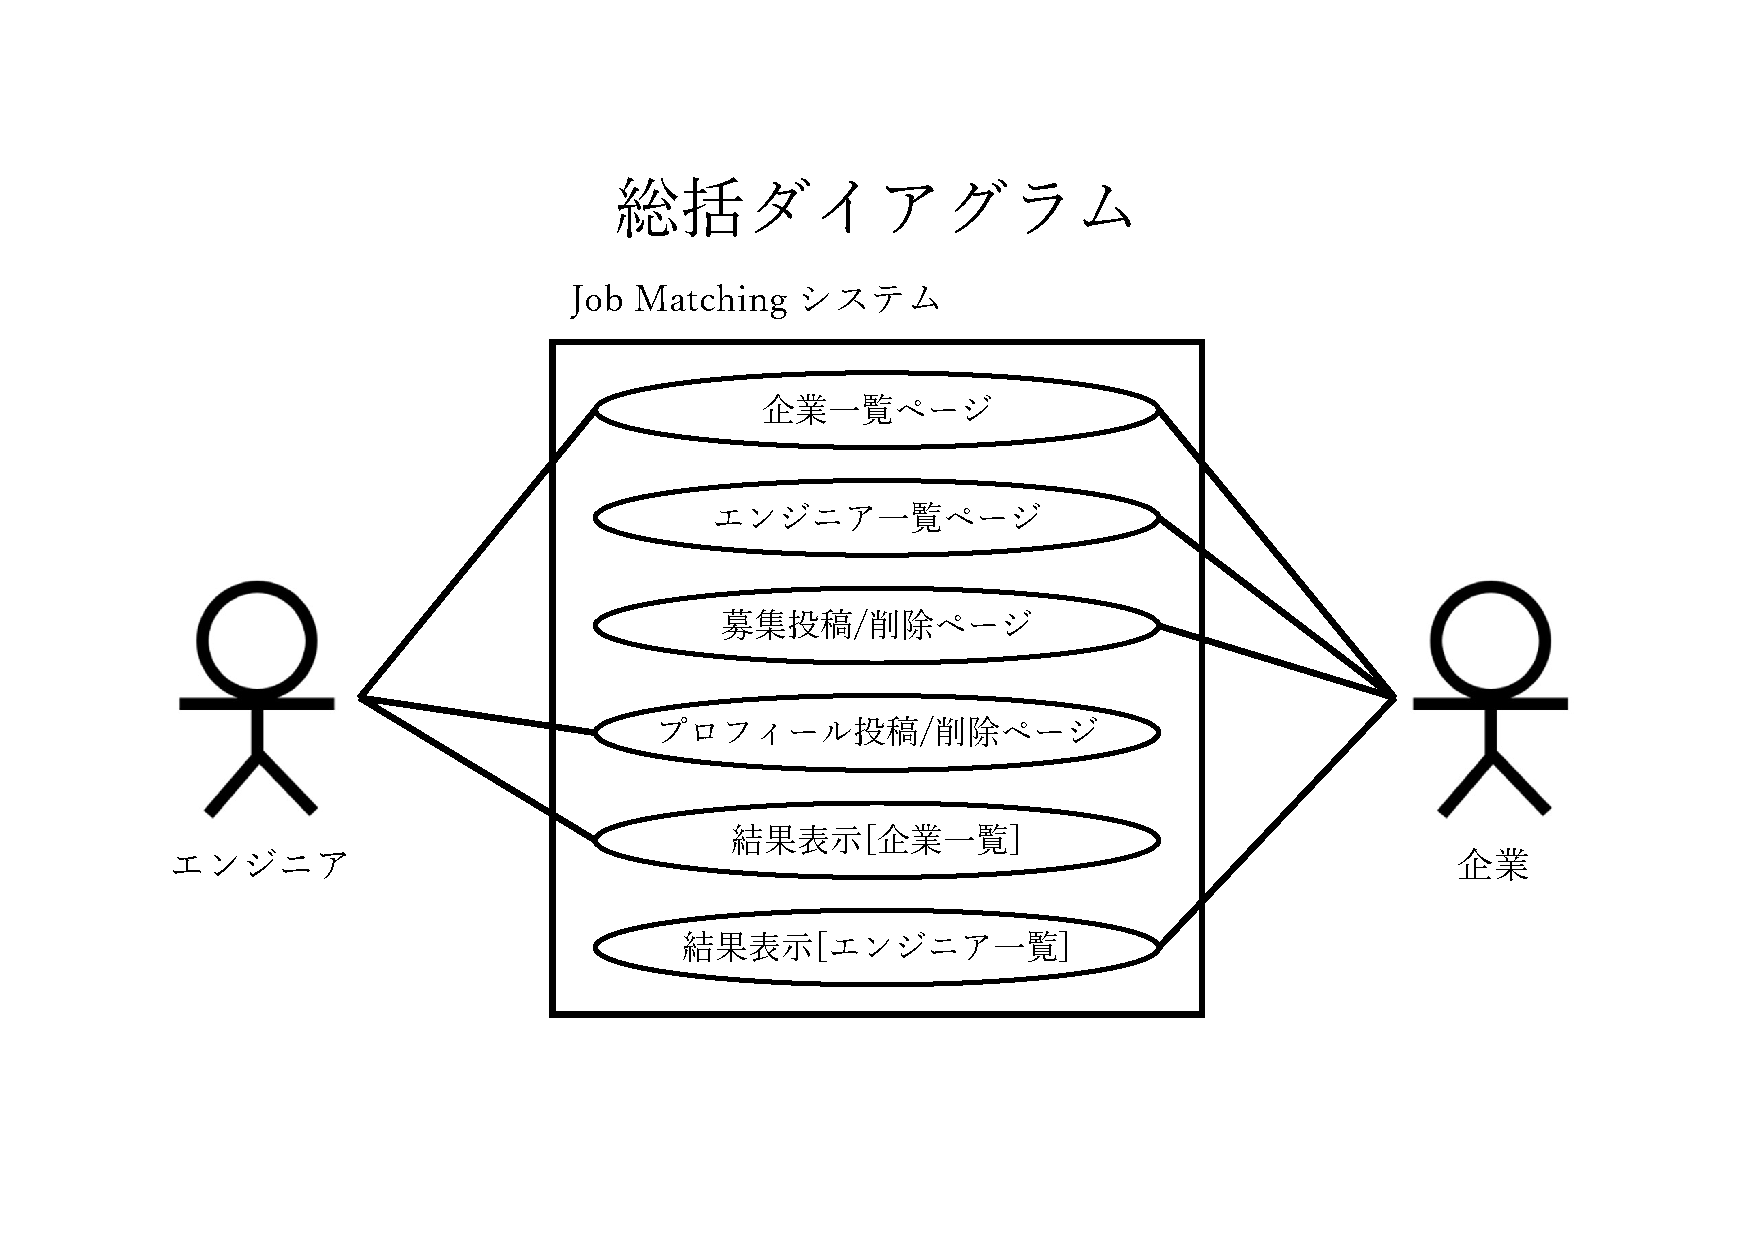
\includegraphics[trim=3cm 3.5cm 3cm 4.7cm, clip, width=14cm]{./img/diagram.pdf}  % 高さを指定して挿入
    \caption{総括ダイアグラム}
    \label{fig:diagram}
\end{figure}
\vspace{-.5cm}

総括ダイアグラムを図\ref{fig:diagram}に示す。\\
\indent 総括ダイアグラムは、エンジニアと企業のマッチングを行うシステムの全体像を示しており、
具体的にどのページにアクセスが可能かどうかを示している。
特徴として、企業側はエンジニアと企業一覧を閲覧することが可能であるが、
エンジニア側は企業一覧のみ閲覧が可能であり、エンジニア一覧を閲覧することはできない。
これは、一般に求人システムにおいてエンジニアは他人の情報を閲覧できないためである。

\newpage
\section{画面遷移詳細}
\begin{figure}[H]
    \centering
    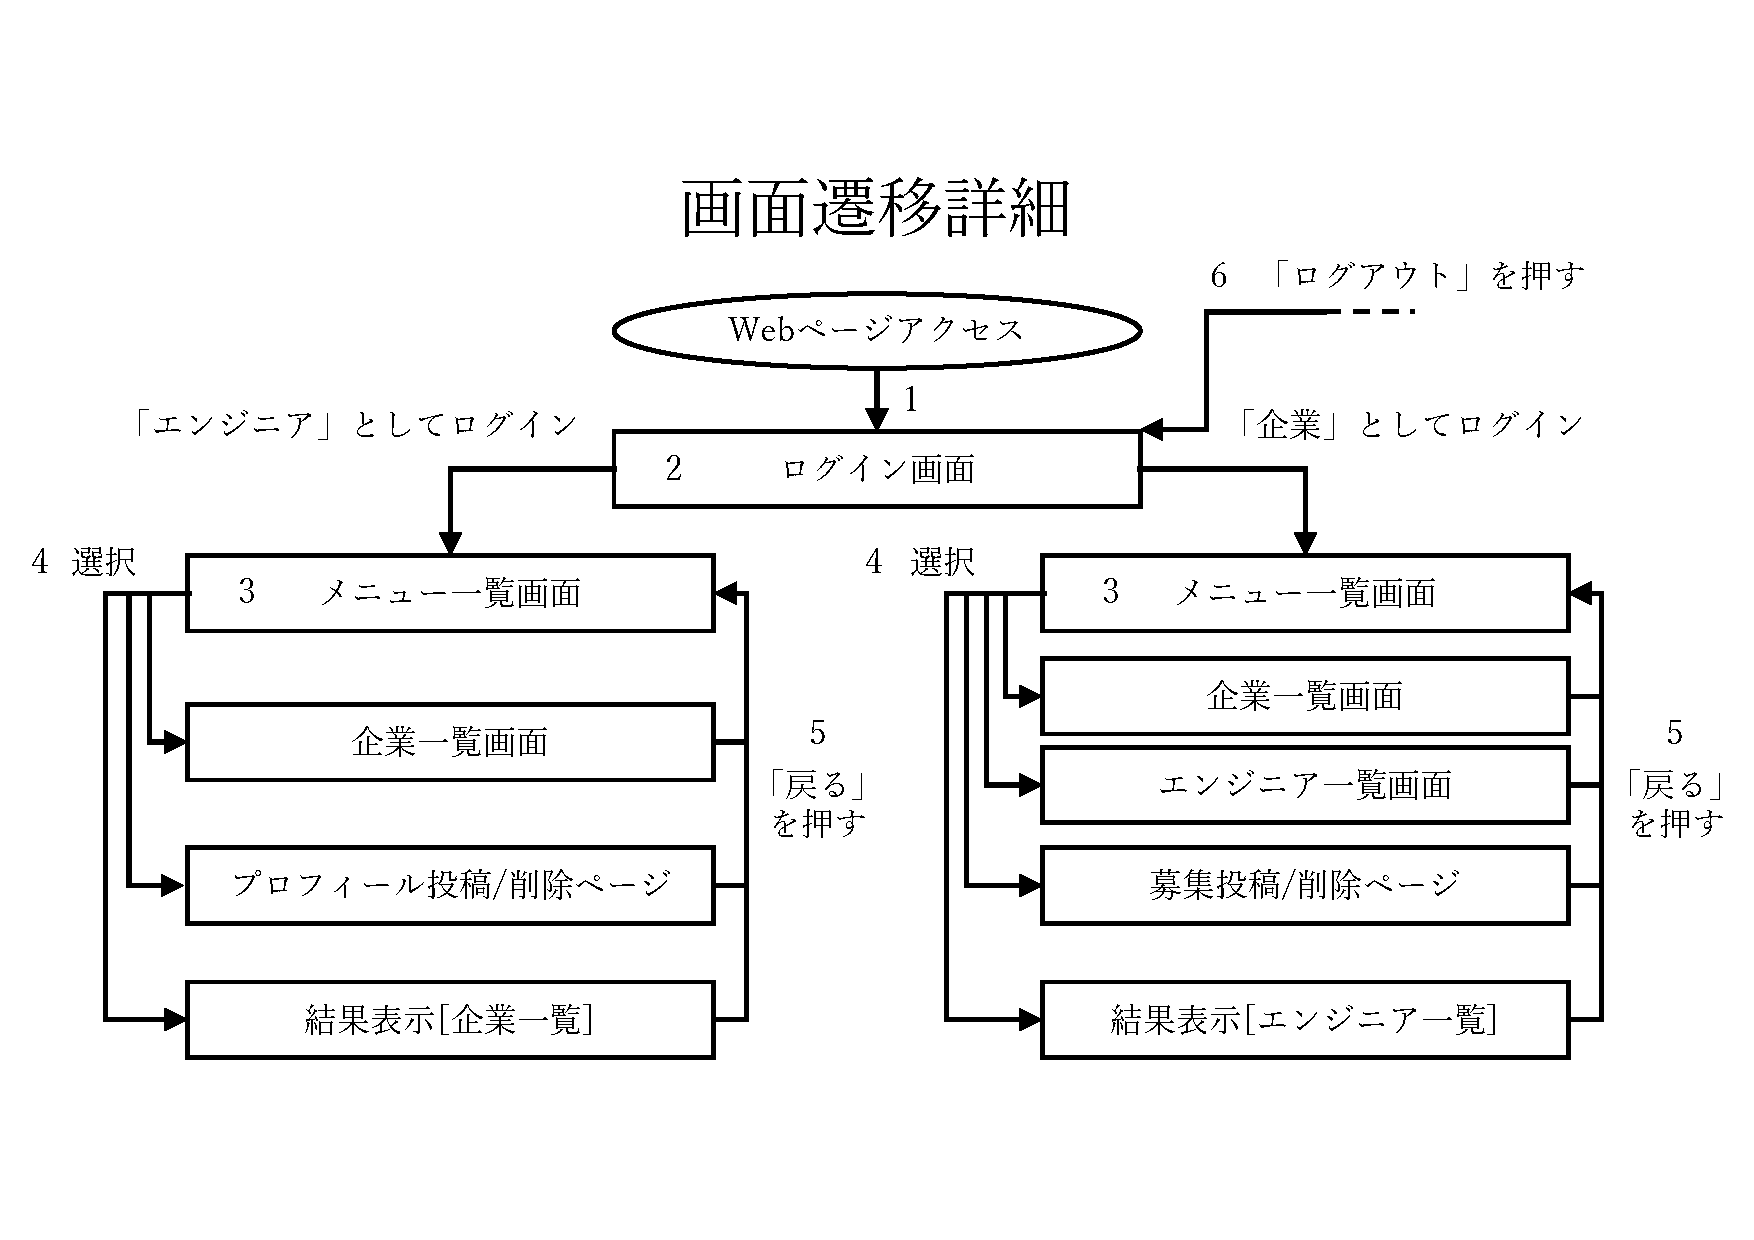
\includegraphics[trim=0.5cm 3cm 0.5cm 4.1cm, clip, width=16cm]{./img/screen_transition.pdf}
    \caption{画面遷移詳細図}
    \label{fig:flow}
\end{figure}
\vspace{-.5cm}

本システムの画面遷移図を図\ref{fig:flow}に示す。\\
\indent 画面遷移図は、ユーザーがどのような操作を行った場合にどのような画面に遷移するかを示している。\\
\indent 以下に、具体的な遷移手順を示す。なお、手順番号は図\ref{fig:flow}中の番号に対応している。\\

\vspace{-0.5cm}
\begin{enumerate}
    \item ユーザーがWebページににアクセスする。
    \begin{enumerate}
        \item 未ログインの場合、ログイン画面に遷移する。(2.へ)
        \item ログイン済みの場合、該当ロール\footnote{ここでのロール(role)は、エンジニア/企業 のいずれかを指す。}
        \footnote{該当ロールとは、以前ログインした際に選択したロールを指す。}
                のメニュー一覧画面に遷移する。(3.へ)
    \end{enumerate}
    \item ログイン画面で、Googleアカウントを用いてログインする。
    \begin{enumerate}
        \item 初回のログインの場合、エンジニア/企業 を選ぶことができ、いずれかのロールを選択可能。
        \item すでに一度Googleアカウントでログインしていた場合、
              以前割り当てられたロールに基づき、エンジニア/企業 いずれかのメニュー一覧画面に遷移する。
    \end{enumerate}
    \item メニュー一覧画面が表示され、それぞれのロールに応じたメニューが表示される。
    \item 各ボタンから、閲覧可能な一覧画面に遷移する。
    \item 各遷移先の画面からは、「戻る」ボタンを押すことで、メニュー一覧画面に戻ることができる。
    \item いずれのページにも、ログアウトボタンが設置されており、ログアウトすることができる。
        ログアウト後は、再度ログイン画面に遷移する。
\end{enumerate}



\newpage
\section{画面レイアウト図}
以下、どちらのロールからの視点かが分かるように、図のタイトルに括弧書きでロール名を記載する。\\
記載がない場合は、共通の画面である。
\subsection{ログイン}
\vspace{-.3cm}
\begin{figure}[H]
    \centering
    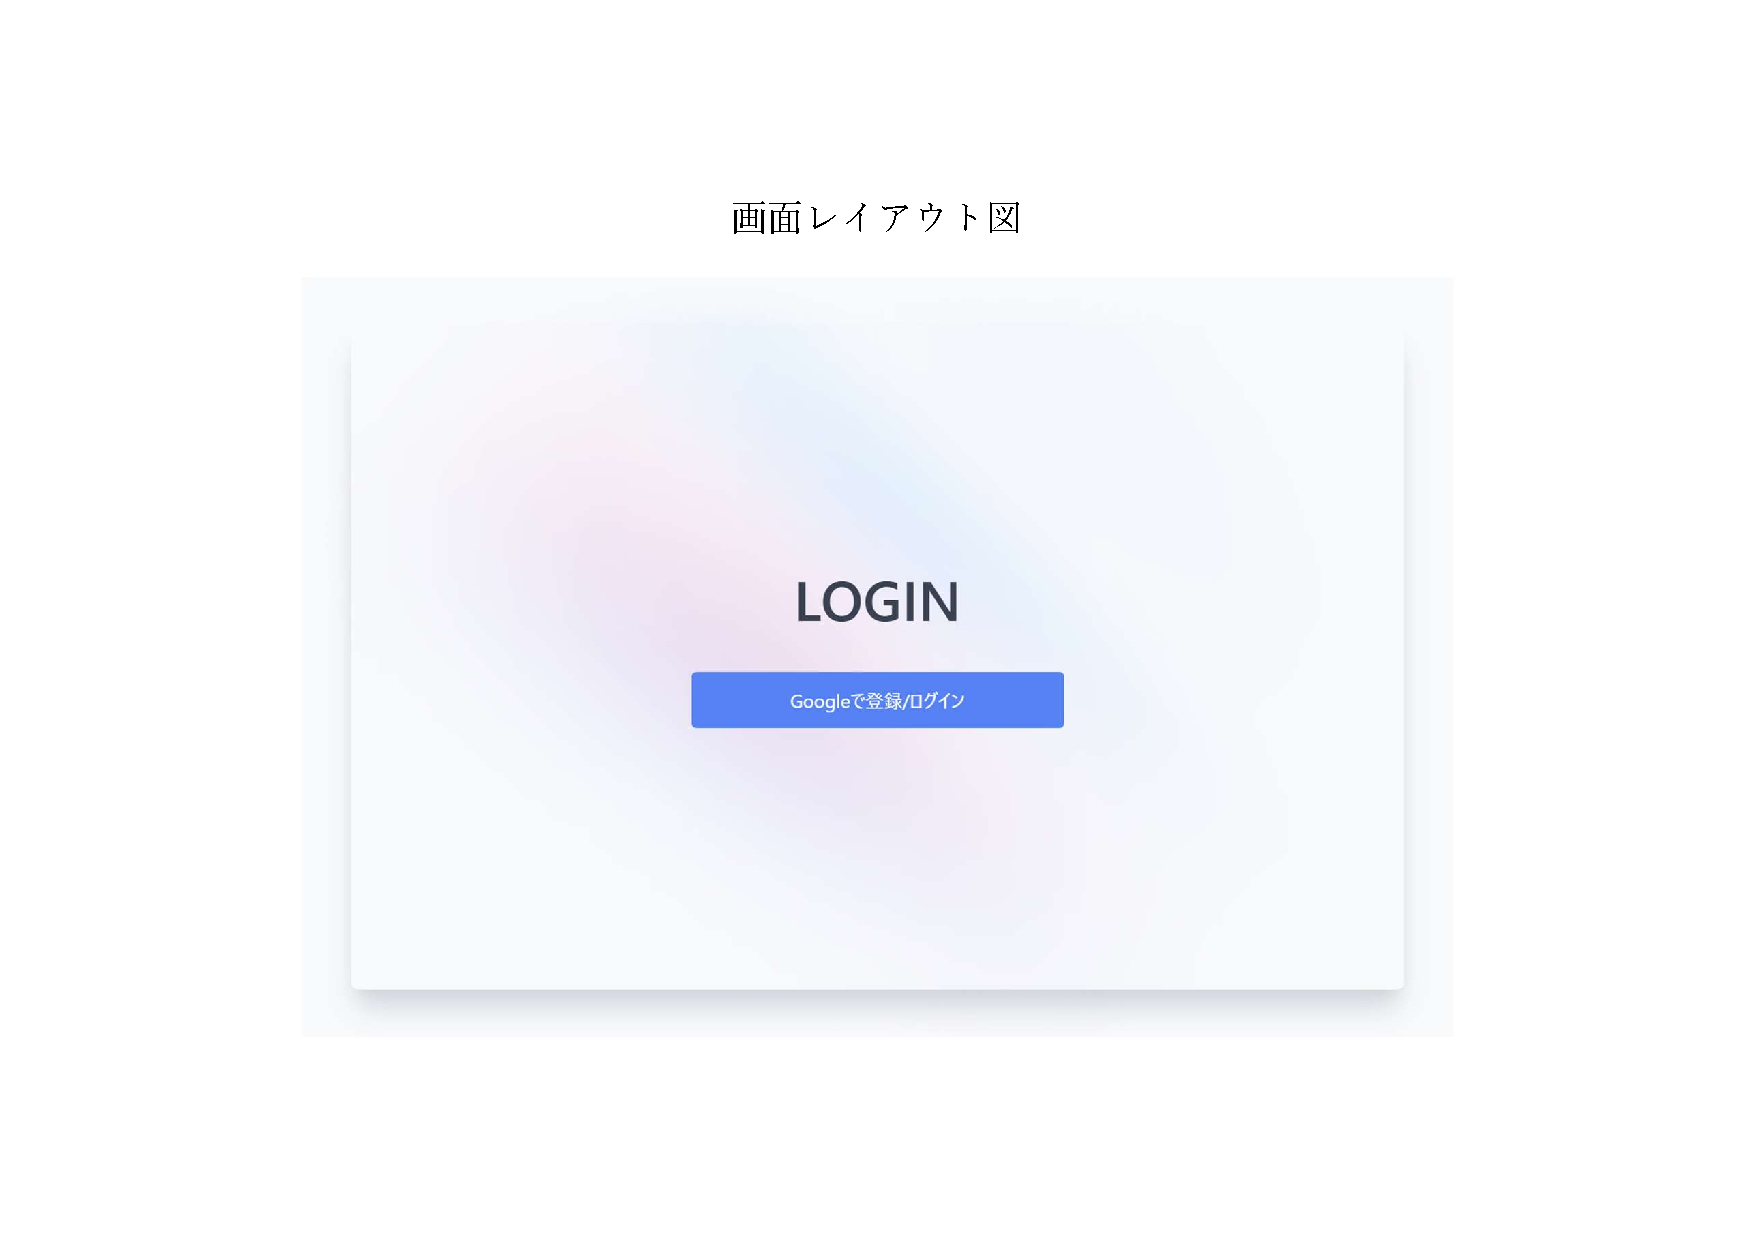
\includegraphics[trim=5.2cm 3.4cm 5.2cm 4.6cm, clip, width=13cm]{./img/login_pages.pdf}
    \caption{ログイン画面}
    \label{fig:login1}
\end{figure}
\vspace{-.6cm}

\begin{figure}[H]
    \centering
    % エンジニアのログイン画面
    \begin{subfigure}{0.49\textwidth}
        \centering
        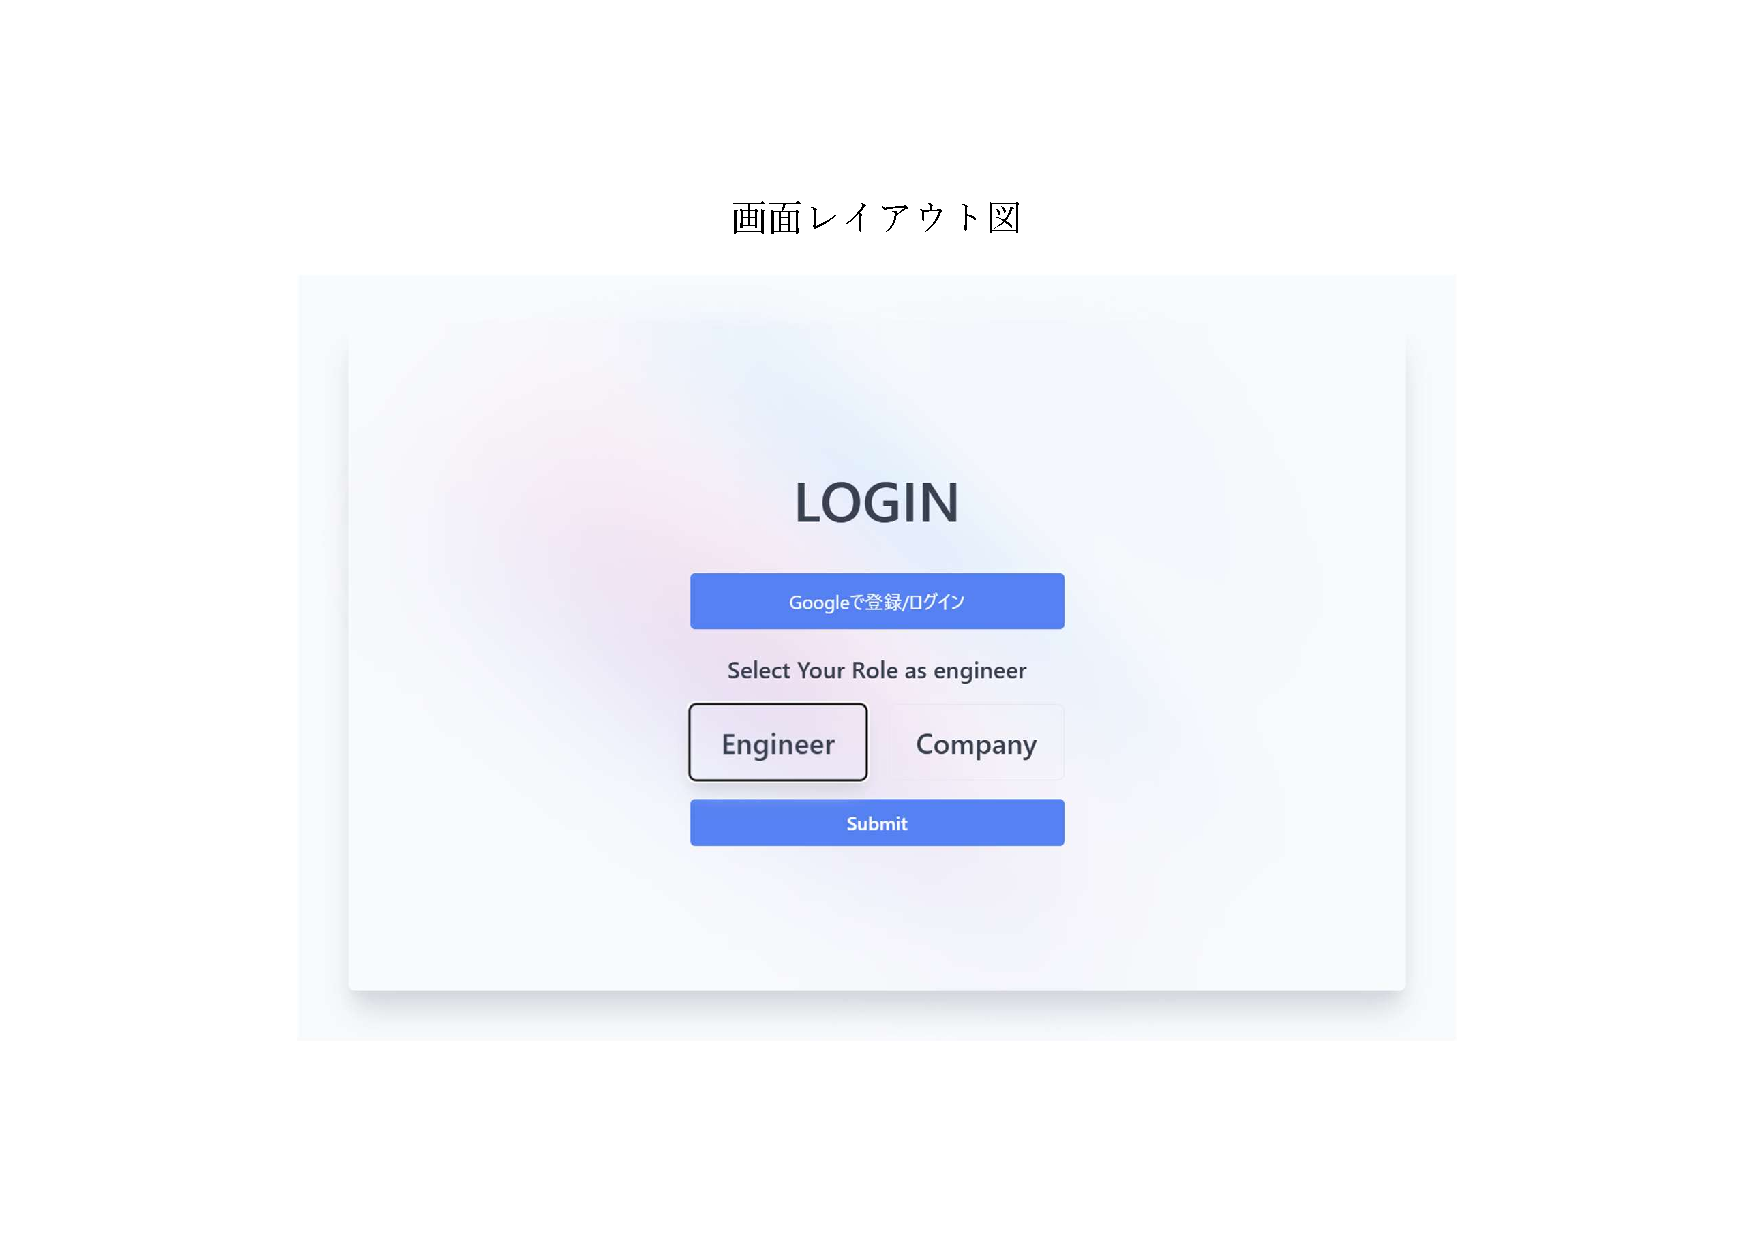
\includegraphics[trim=5.2cm 3.4cm 5.2cm 4.6cm, clip, width=\linewidth]{./img/login_pages_engineer.pdf}
        \caption{エンジニアとして登録}
        \label{fig:login_engineer}
    \end{subfigure}
    \hfill
    % 企業のログイン画面
    \begin{subfigure}{0.49\textwidth}
        \centering
        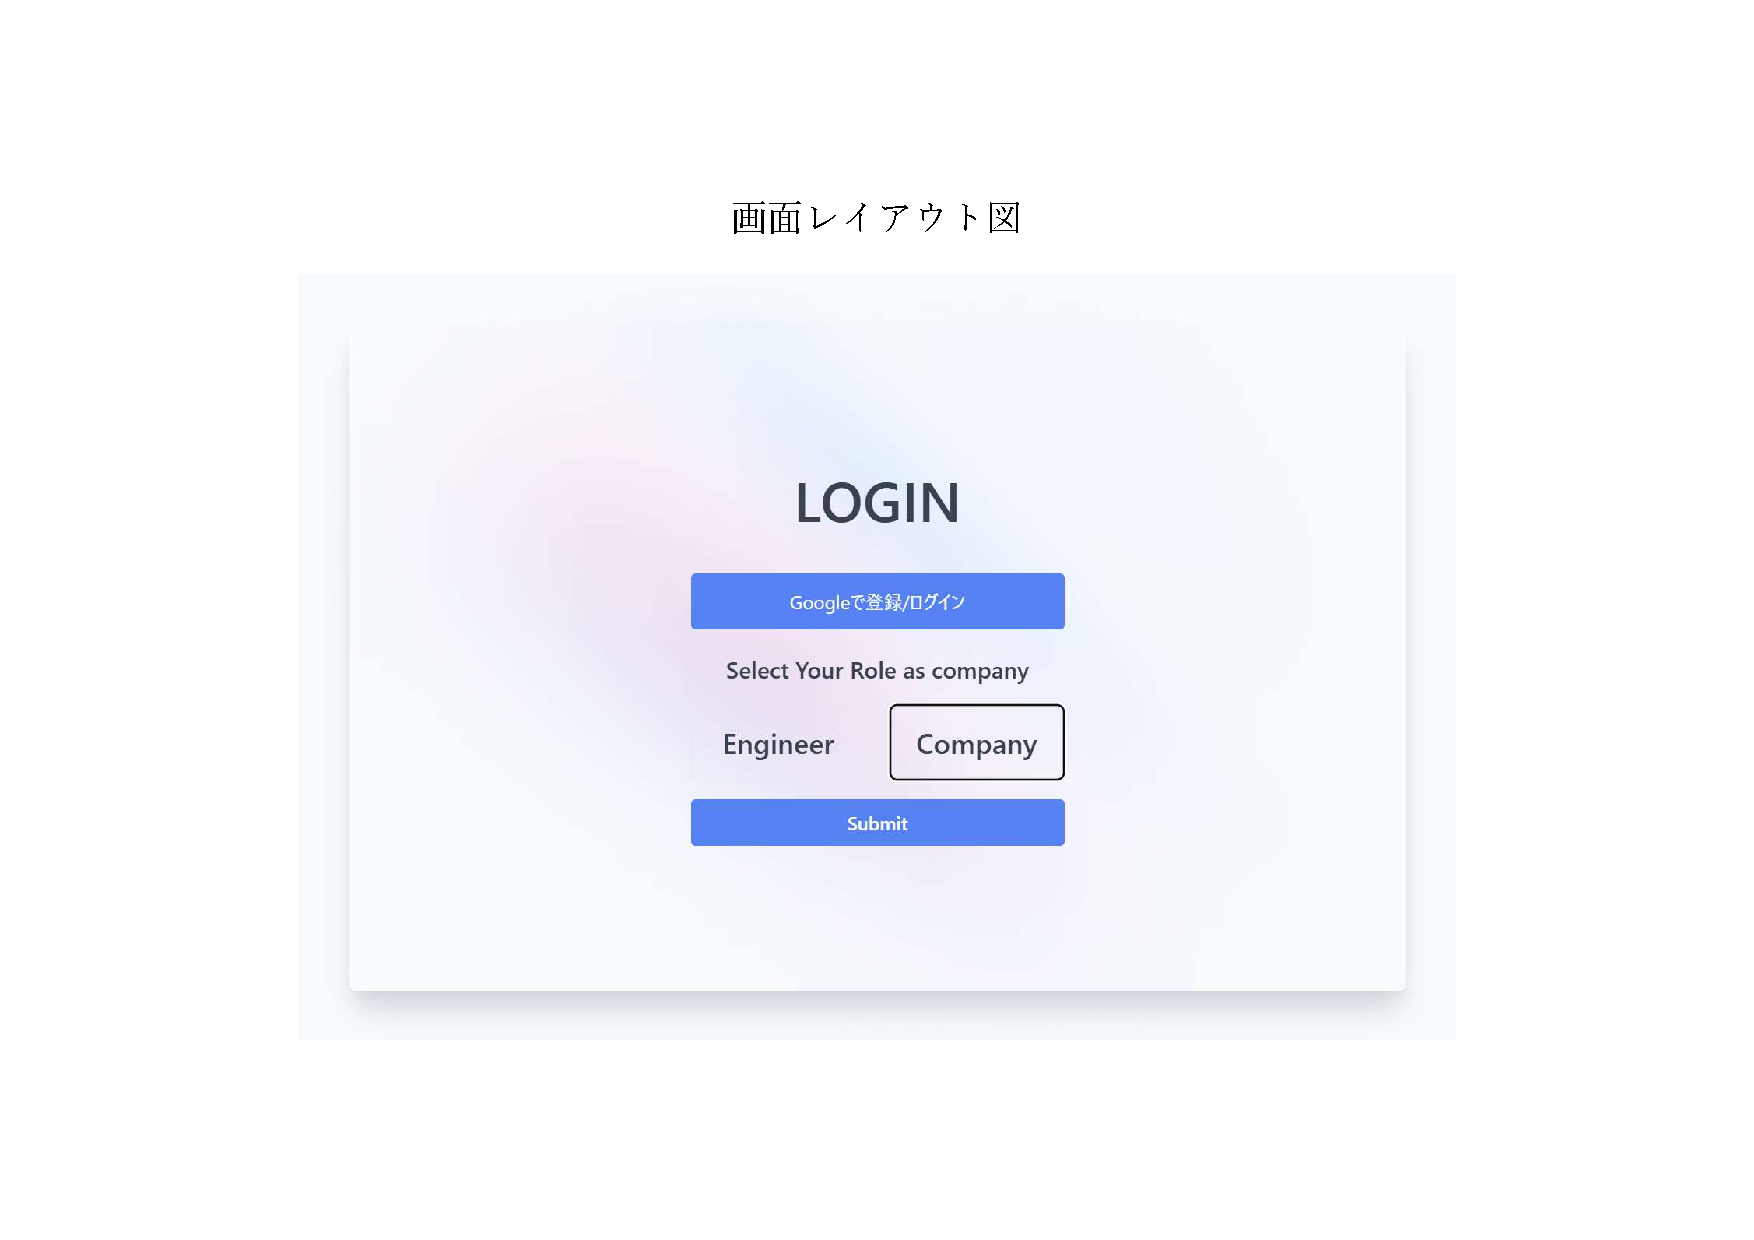
\includegraphics[trim=5.2cm 3.4cm 5.2cm 4.6cm, clip, width=\linewidth]{./img/login_pages_company.pdf}
        \caption{企業として登録}
        \label{fig:login_company}
    \end{subfigure}
    \caption{初回登録画面}
    \label{fig:register}
\end{figure}
\vspace{-.5cm}

図\ref{fig:login1}は、ログイン画面を示している。Googleで登録/ログイン ボタンを押すと、
Googleアカウントでログインするフォームが表示され、ログインすることができる。\\
\indent この操作の後、手順2(a)のような初回ログインの場合、図\ref{fig:register}(a), 図\ref{fig:register}(b)のように、
いずれかを選択するフォームが表示される。この選択により、Googleアカウントに 企業/エンジニア の情報が紐づけられ、
次回以降のログイン時には、選択したロールに基づいてメニュー一覧画面に遷移(手順2(b))する。
\newpage
\subsection{メニュー一覧}
\begin{figure}[H]
    \centering
    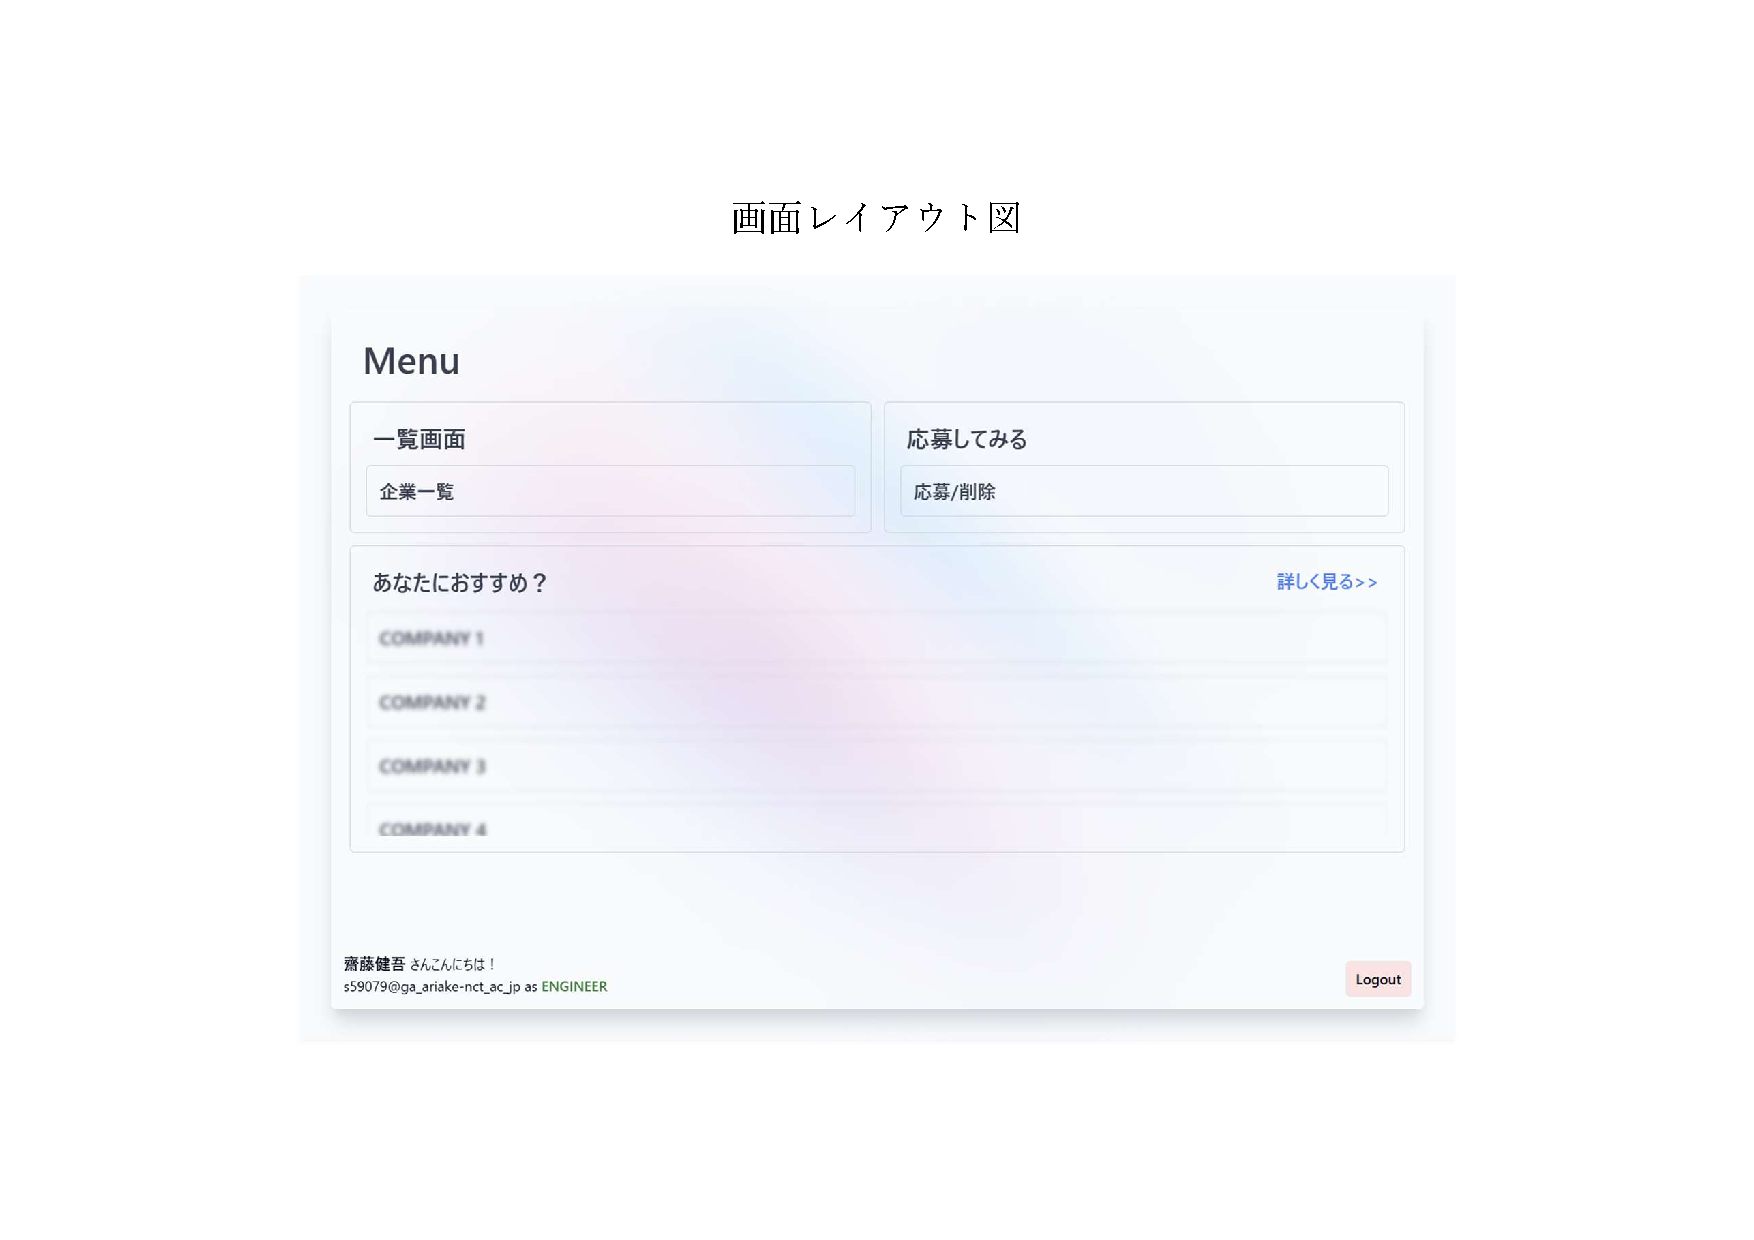
\includegraphics[trim=5.2cm 3.4cm 5.2cm 4.7cm, clip, width=13.5cm]{./img/menu_pages_engineer.pdf}
    \caption{メニュー一覧画面(エンジニア)}
    \label{fig:menu_engineer}
\end{figure}
\vspace{-.7cm}

\begin{figure}[H]
    \centering
    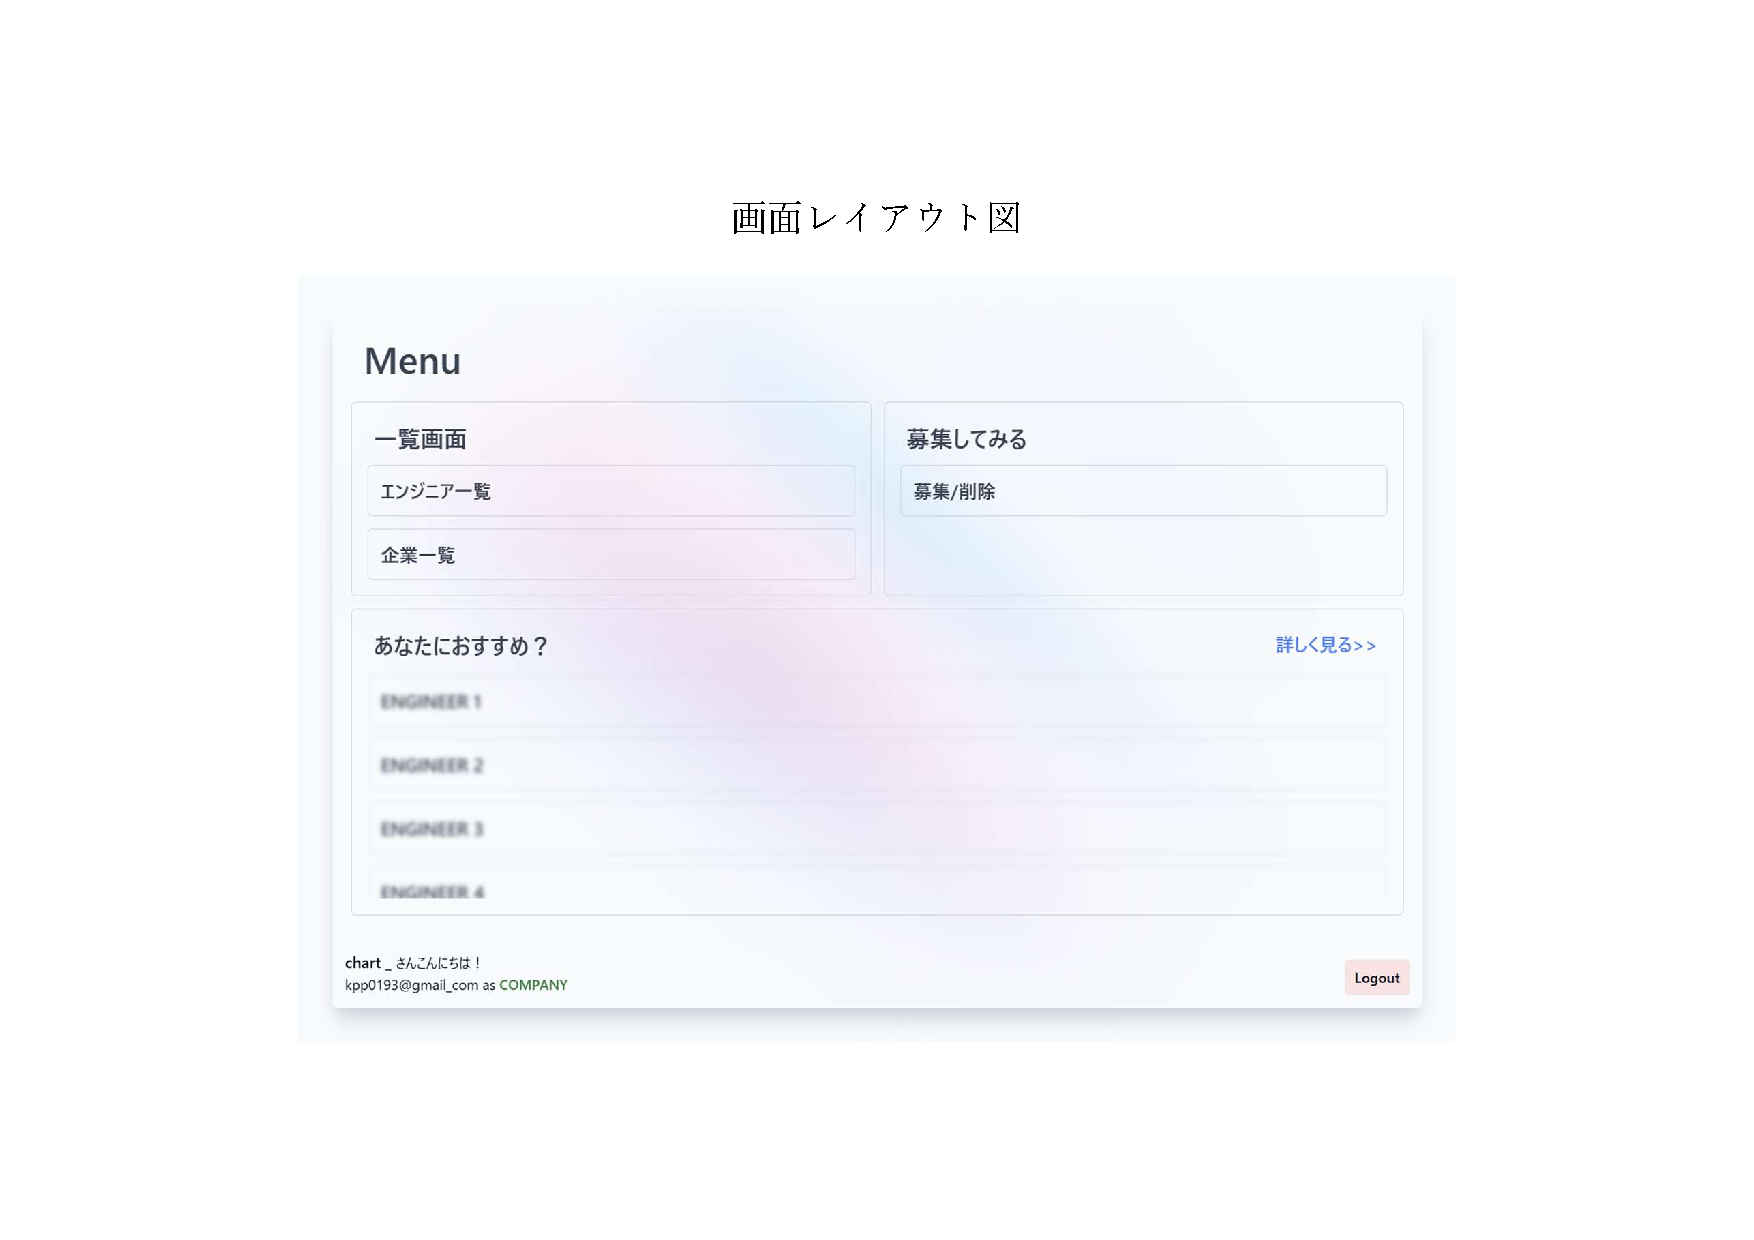
\includegraphics[trim=5.2cm 3.4cm 5.2cm 4.7cm, clip, width=13.5cm]{./img/menu_pages_company.pdf}
    \caption{メニュー一覧画面(企業)}
    \label{fig:menu_company}
\end{figure}
\vspace{-.5cm}

図\ref{fig:menu_engineer}は、エンジニアとしてログインした際のメニュー一覧画面を示しており、
図\ref{fig:menu_company}は、企業としてログインした際のメニュー一覧画面を示している。\\
\indent 2.総括ダイアグラムに示した通り、エンジニアは企業一覧画面のみ閲覧可能であり、
企業はエンジニア一覧画面と企業一覧画面の両方が閲覧可能である。
このボタンを押すと、図\ref{fig:list_engineer}, 図\ref{fig:list_company}のような一覧画面に遷移する。\\
\indent "募集してみる" 内のボタンを押すと、図\ref{fig:form_engineer}, 図\ref{fig:form_company}
のような応募画面に遷移する。\\
\indent "あなたにおすすめ?" の右側 「詳しく見る>>」ボタンを押すと、
図\ref{fig:recommend_engineer1}, 図\ref{fig:recommend_company1}
のようなマッチング画面に遷移する。\\
\indent 画面左下には、Googleアカウントに紐づいたユーザー名・メールアドレスに加え、ロールが表示されており、
現在どのアカウントでログインしているか、自身のロールが何かを一目で分かるようになっている。\\
\indent また、画面右下には、ログアウトボタンが設置されており、ログアウトすることができる。
このボタンは、ログインページ以外の全てのページに設置されている。
\newpage
\subsection{応募/求人一覧画面}
\begin{figure}[H]
    \centering
    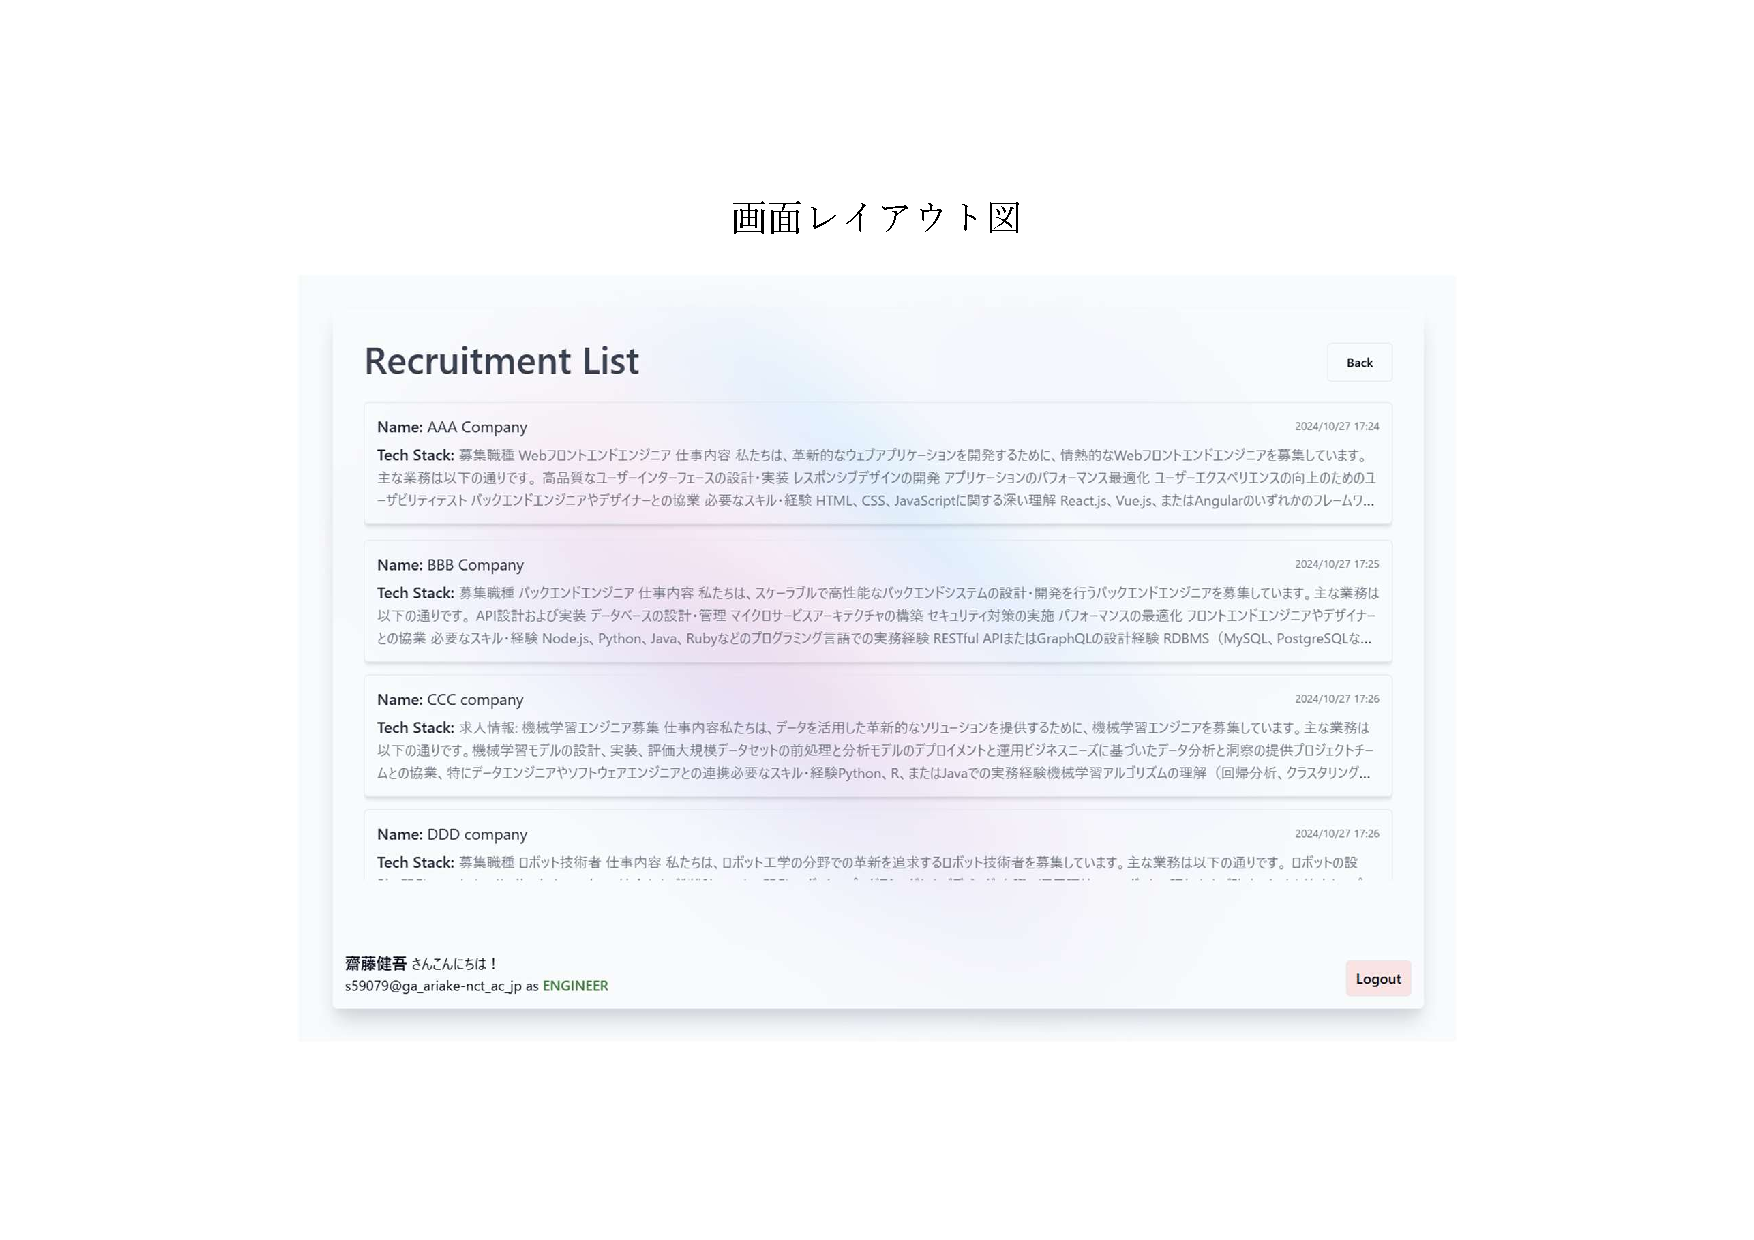
\includegraphics[trim=5.2cm 3.4cm 5.2cm 4.6cm, clip, width=14cm]{./img/List_pages_engineer.pdf}
    \caption{企業一覧画面(エンジニア)}
    \label{fig:list_engineer}
\end{figure}
\vspace{-.5cm}


\begin{figure}[H]
    \centering
    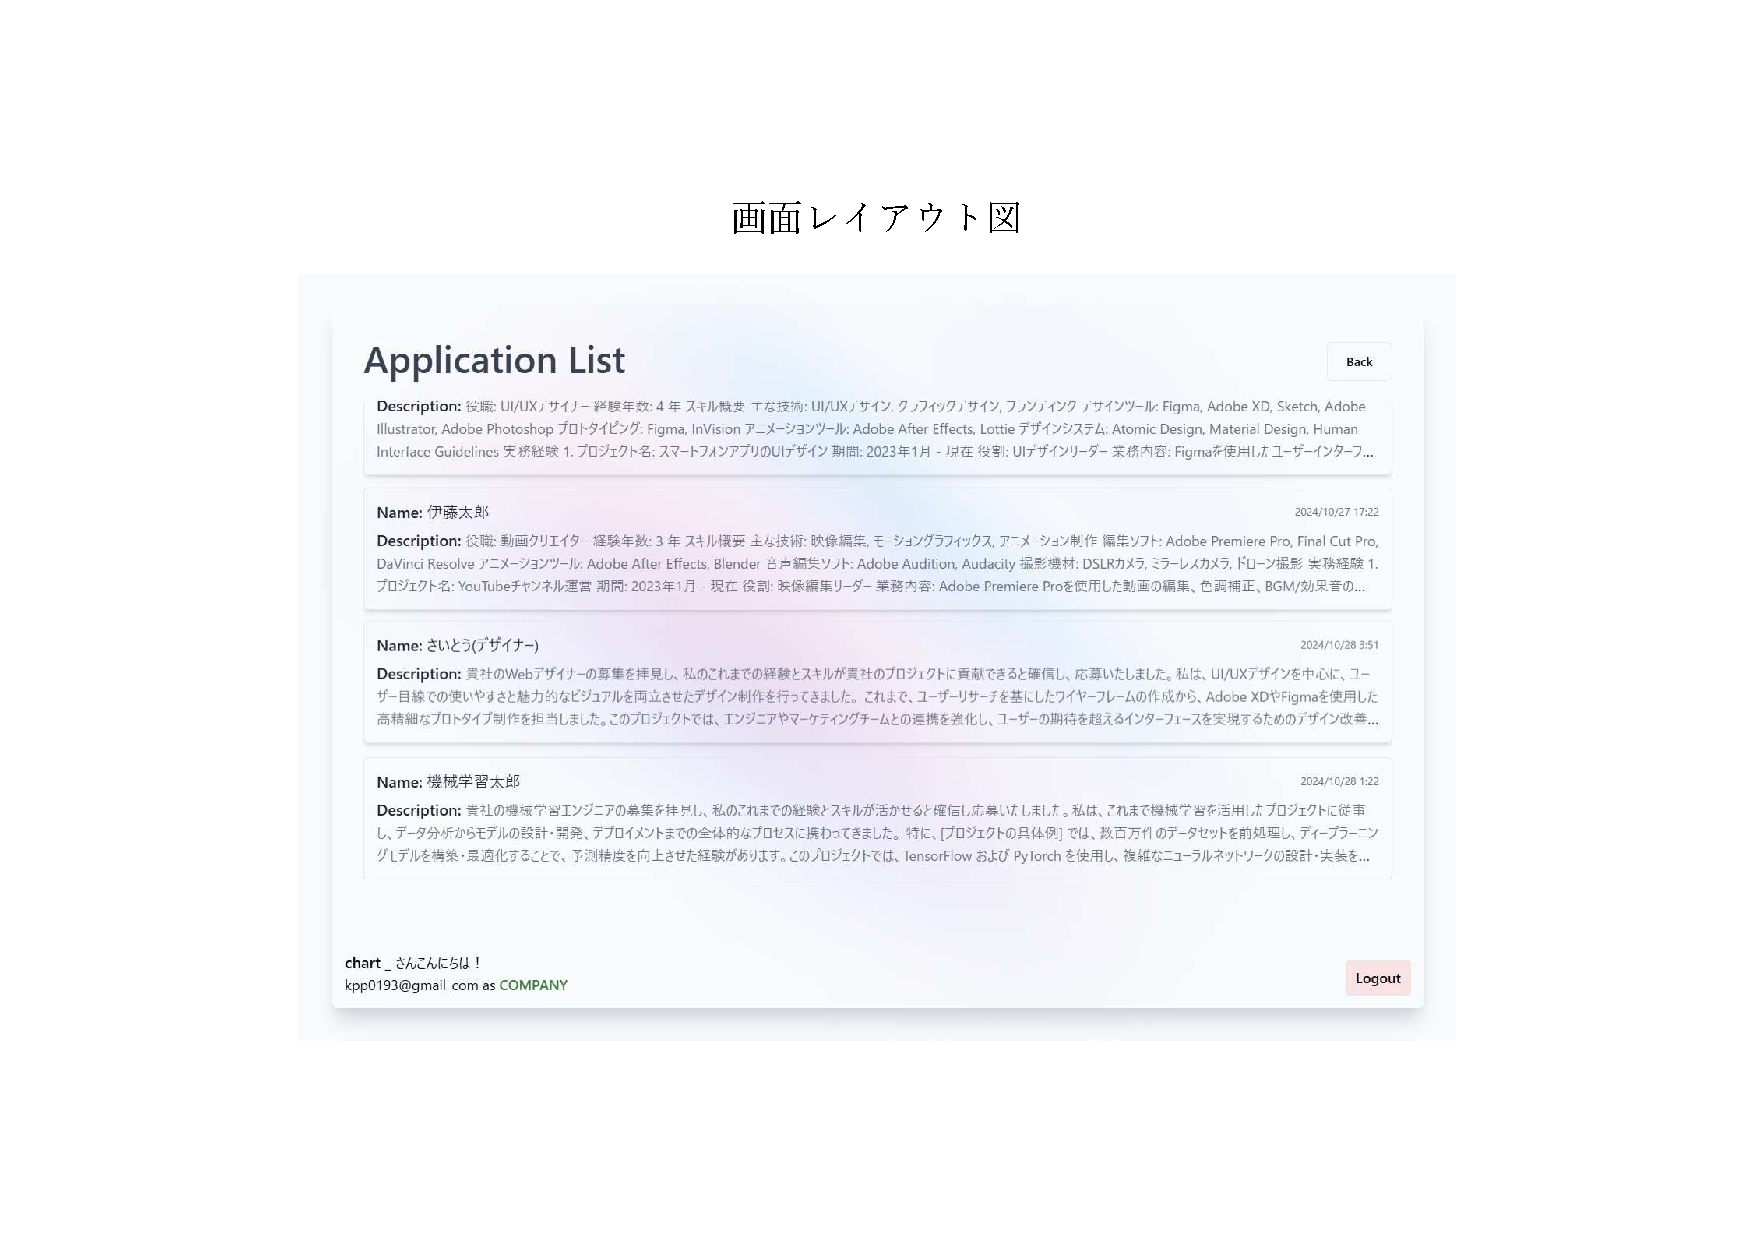
\includegraphics[trim=5.2cm 3.4cm 5.2cm 4.6cm, clip, width=14cm]{./img/List_pages_company.pdf}
    \caption{エンジニア一覧画面(企業)}
    \label{fig:list_company}
\end{figure}
\vspace{-.5cm}

\begin{figure}[H]
    \centering
    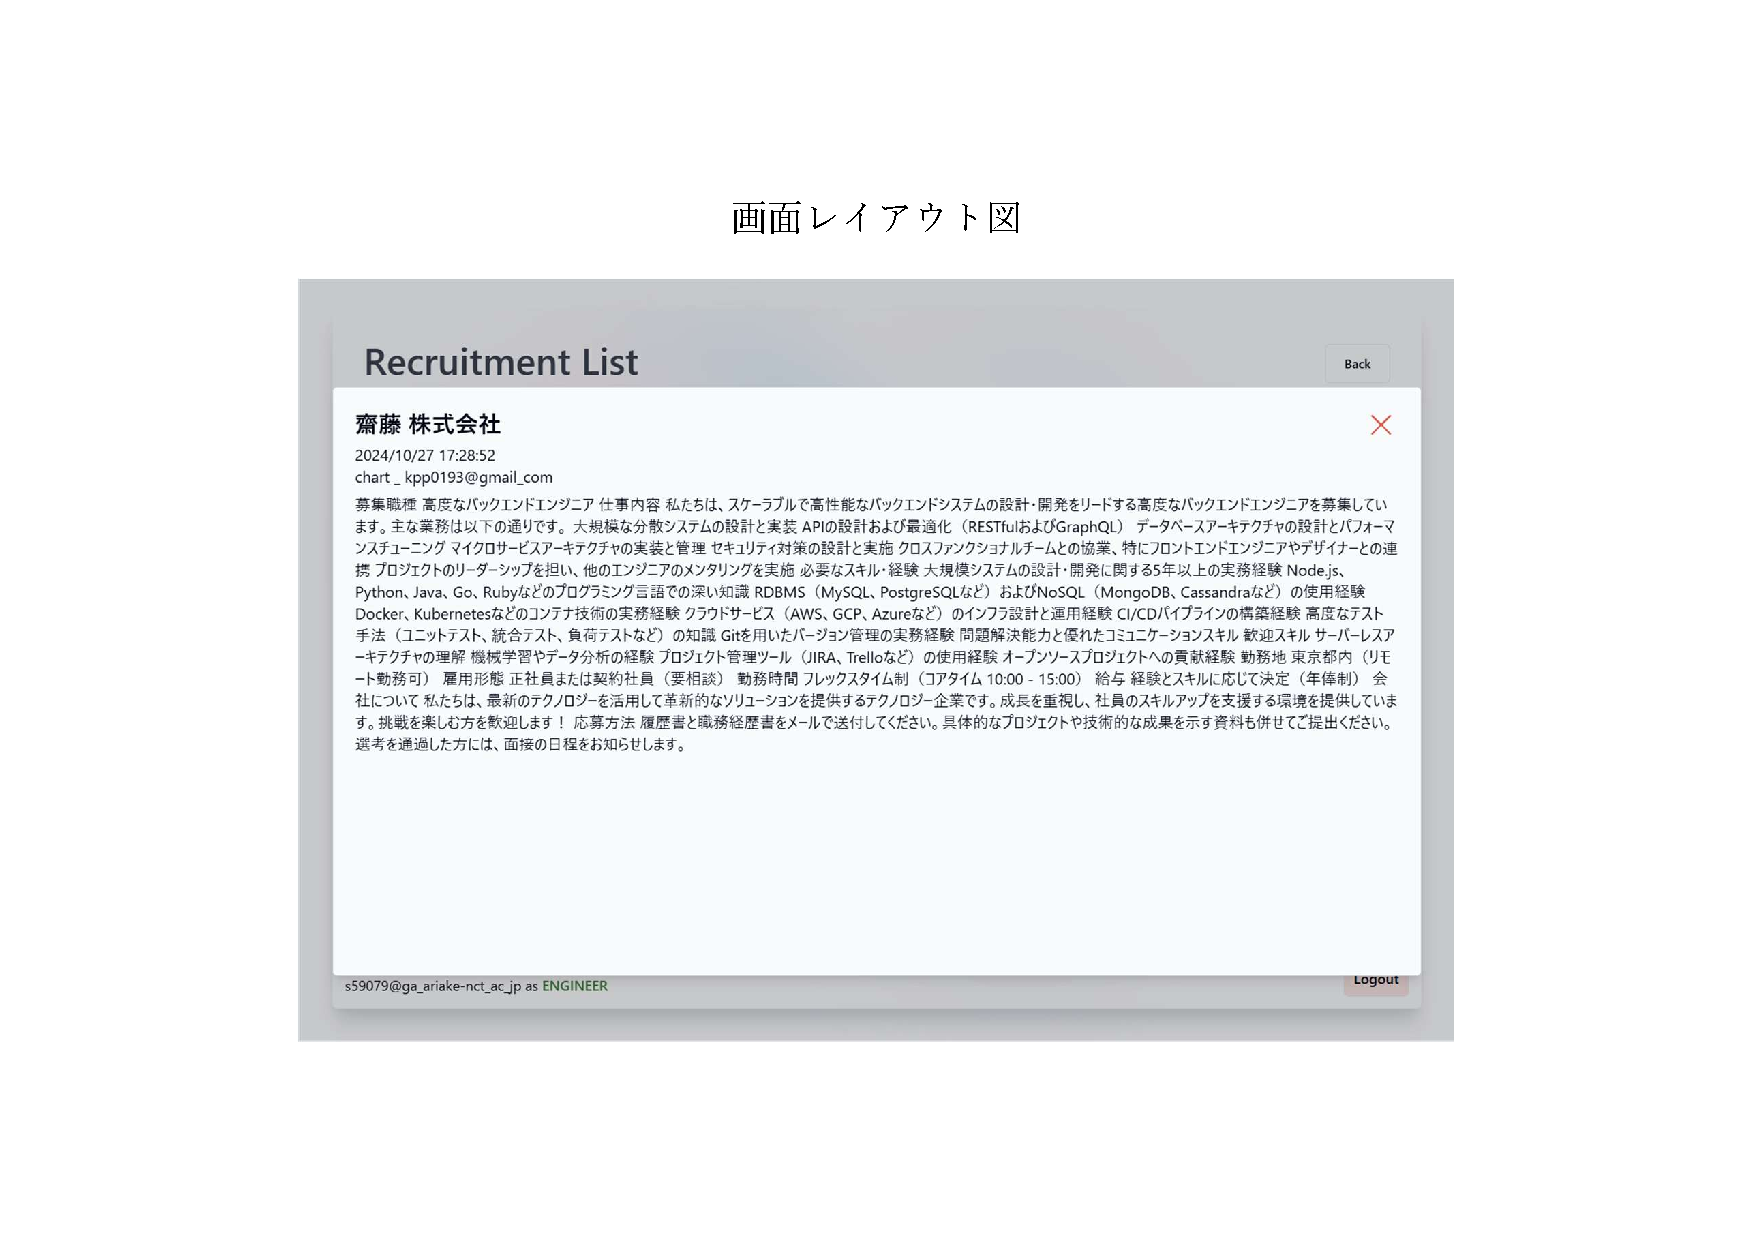
\includegraphics[trim=5.2cm 3.4cm 5.2cm 4.6cm, clip, width=14cm]{./img/List_pages_engineer_detail.pdf}
    \caption{一覧詳細(共通)}
    \label{fig:list_engineer_details}
\end{figure}
\vspace{-.5cm}

図\ref{fig:list_engineer}は、エンジニアが企業一覧画面を表示した際の画面を示しており、
図\ref{fig:list_company}は、企業がエンジニア一覧画面を表示した際の画面を示している。\\
\indent これらのページは、後に示す応募/募集画面から投稿された情報を表示するためのページである。
また、それぞれのデータには、投稿者の名前、投稿日時、本文が表示され、
全て表示されるのではなく、3行で省略され、大きさが統一されている。データの詳細を見るためには、
そのデータをクリックすることで、図\ref{fig:list_engineer_details}のような詳細画面に遷移し、
先ほど表示されていた情報に加え、Gmailの名前、Gmailアドレス、全ての本文が表示される。\\
右上の $\times$ ボタンを押すと、このポップアップは消え、先ほどの画面に戻る。

\newpage
\subsection{応募/募集画面}
\begin{figure}[H]
    \centering
    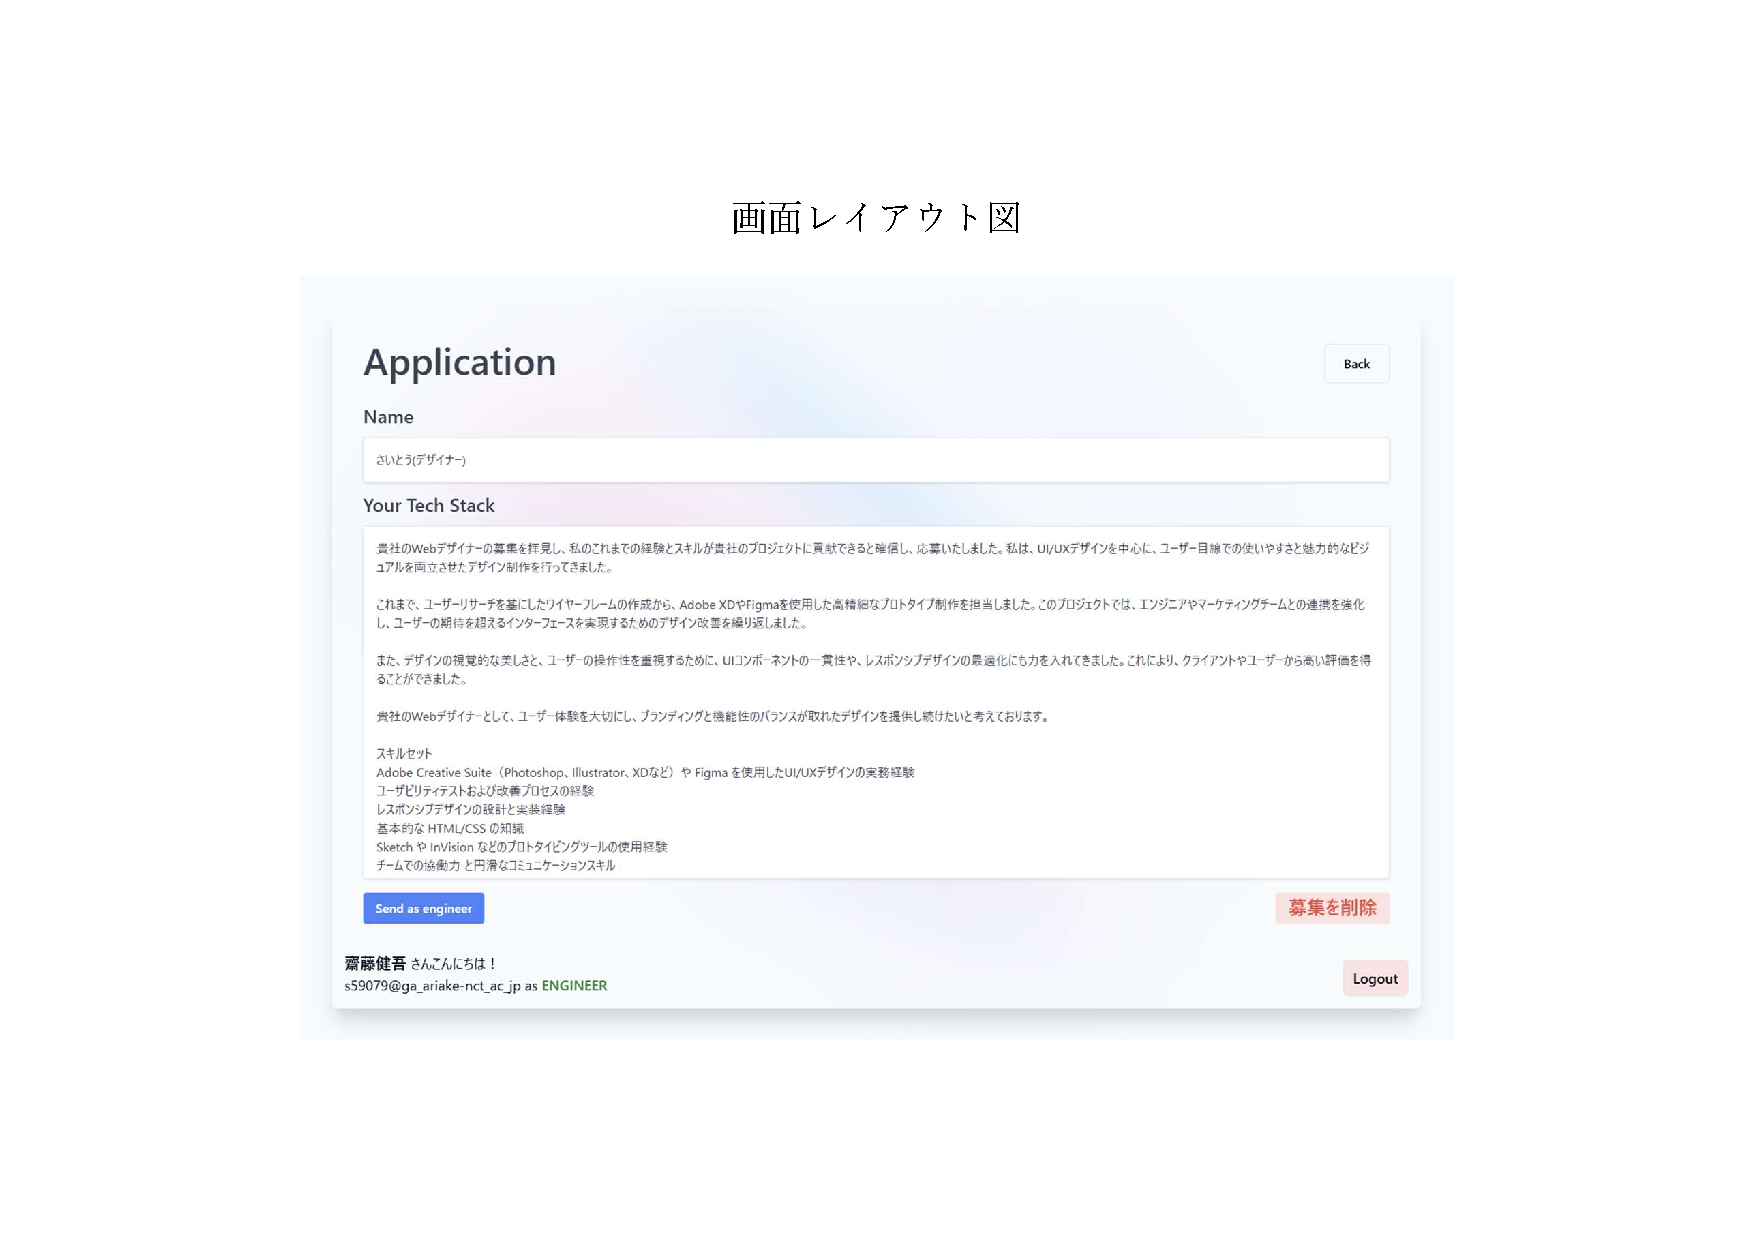
\includegraphics[trim=5.2cm 3.4cm 5.2cm 4.6cm, clip, width=14cm]{./img/Form_pages_engineer.pdf}
    \caption{応募画面(エンジニア)}
    \label{fig:form_engineer}
\end{figure}
\vspace{-.5cm}

\begin{figure}[H]
    \centering
    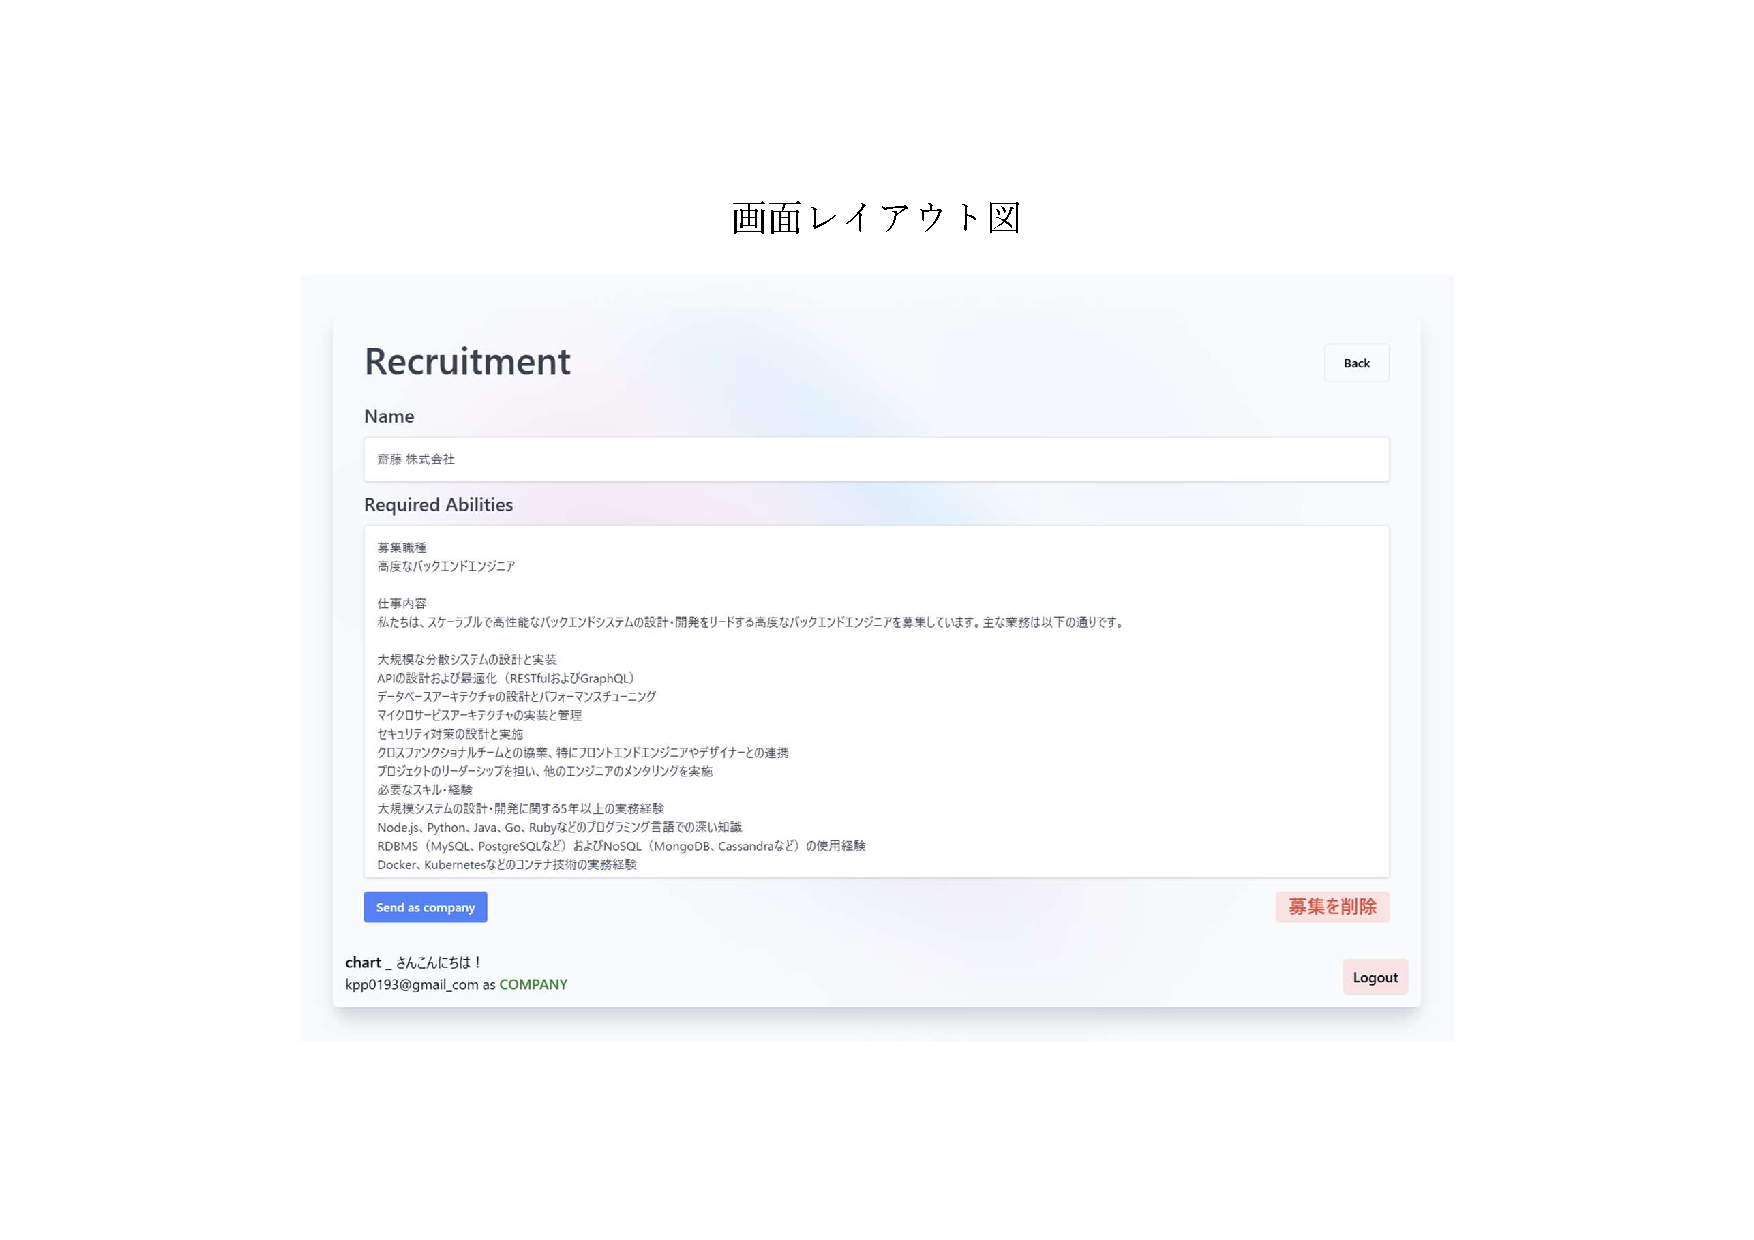
\includegraphics[trim=5.2cm 3.4cm 5.2cm 4.6cm, clip, width=14cm]{./img/Form_pages_company.pdf}
    \caption{募集画面(企業)}
    \label{fig:form_company}
\end{figure}
\vspace{-.5cm}

図\ref{fig:form_engineer}は、エンジニアが応募画面を表示した際の画面を示しており、
図\ref{fig:form_company}は、企業が募集画面を表示した際の画面を示している。\\
\indent 一度投稿した情報は、企業一覧画面、エンジニア一覧画面に表示され、
既に自分のアカウントから投稿されていれば、フォームに一から入力することなく、編集することができる。\\
現在、自分のアカウントから投稿されている情報があれば、右下の「募集を削除」ボタンを押すことができ、
その情報を削除することができる。\\
エンジニアと企業でのUIの違いは、左下の情報と表示する文字の違い(ヘッダのApplication/Recruitment や ボタン Send as \_ など)であり、
本質的な機能に違いはない。

\newpage
\subsection{マッチング画面}
\begin{figure}[H]
    \centering
    \begin{subfigure}{0.49\textwidth}
        \centering
        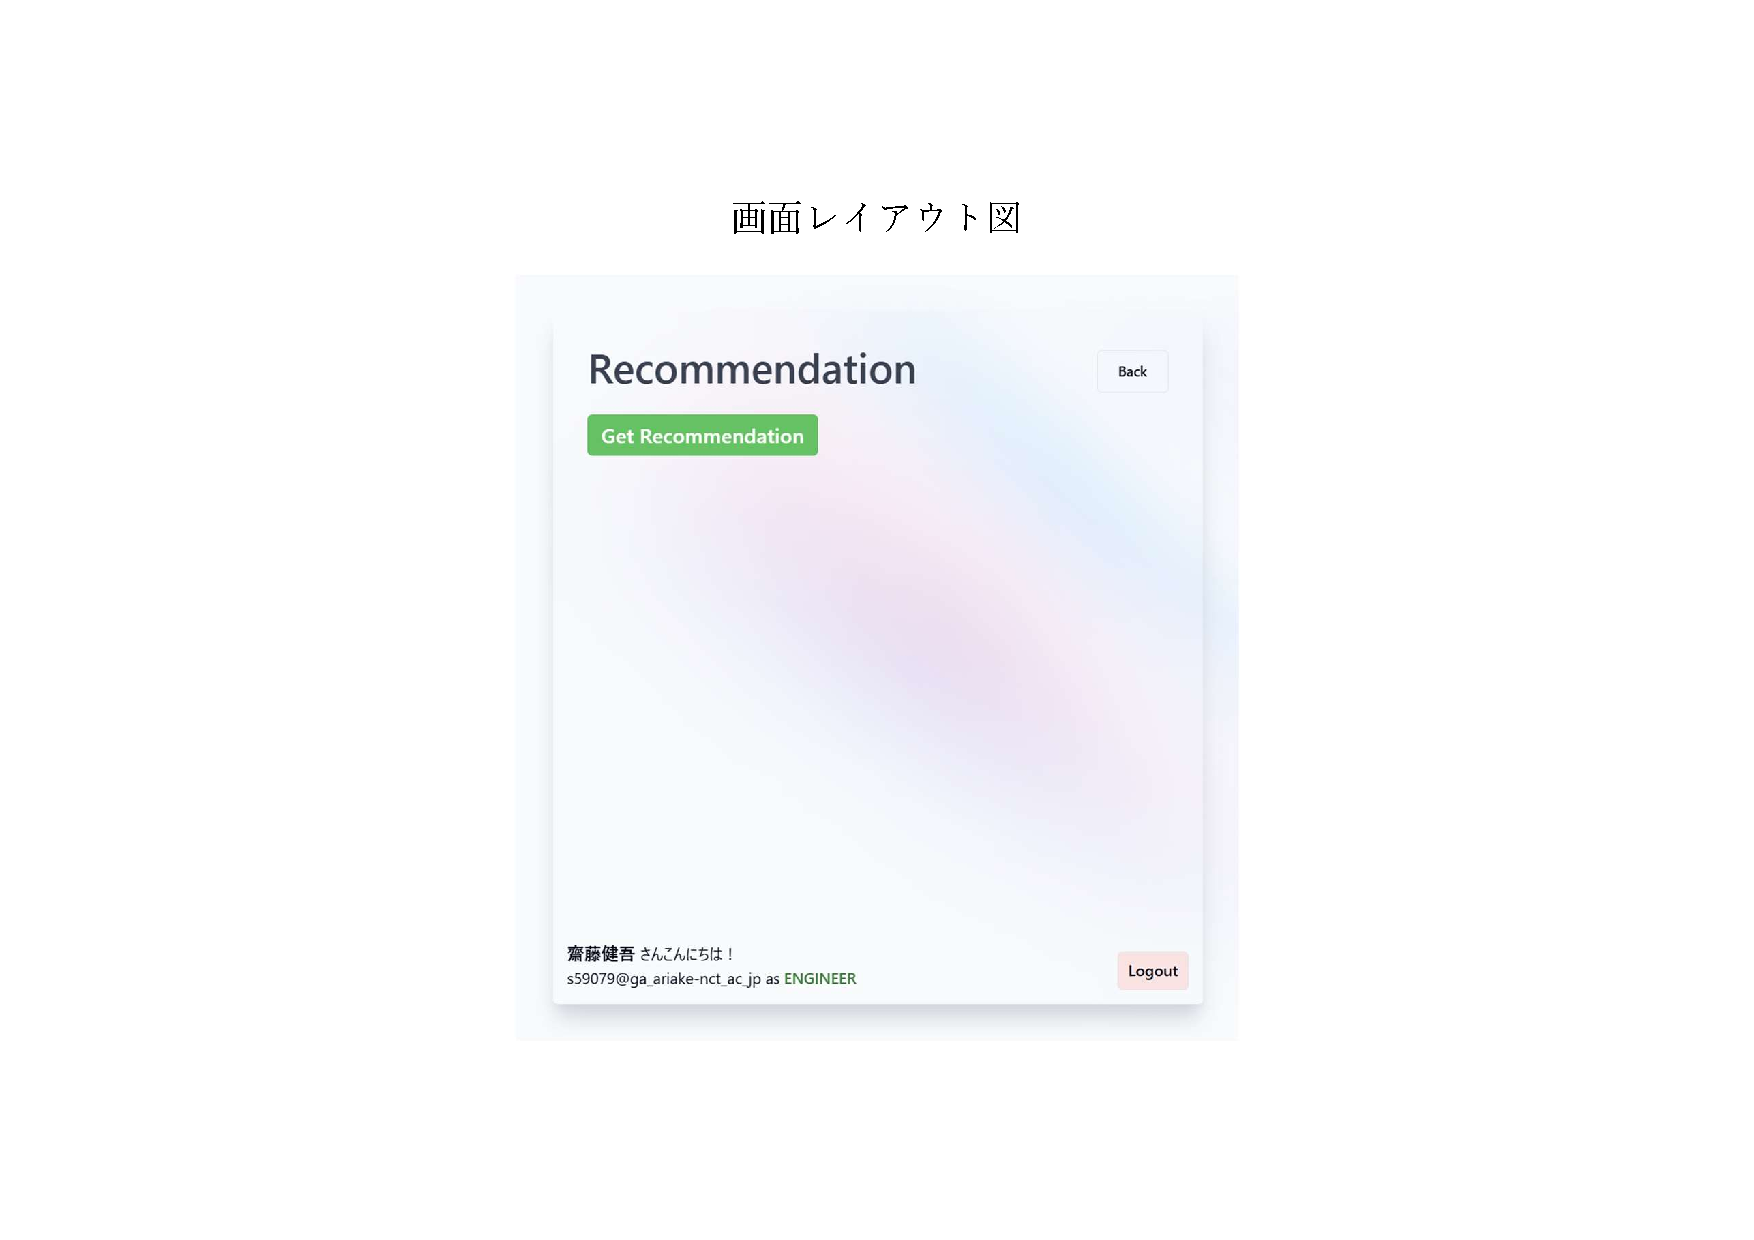
\includegraphics[trim=9cm 3.4cm 9cm 4.6cm, clip, width=\linewidth]{./img/recommend_engineer1.pdf}
        \caption{マッチング画面(エンジニア)}
        \label{fig:recommend_engineer1}
    \end{subfigure}
    \hfill
    \begin{subfigure}{0.49\textwidth}
        \centering
        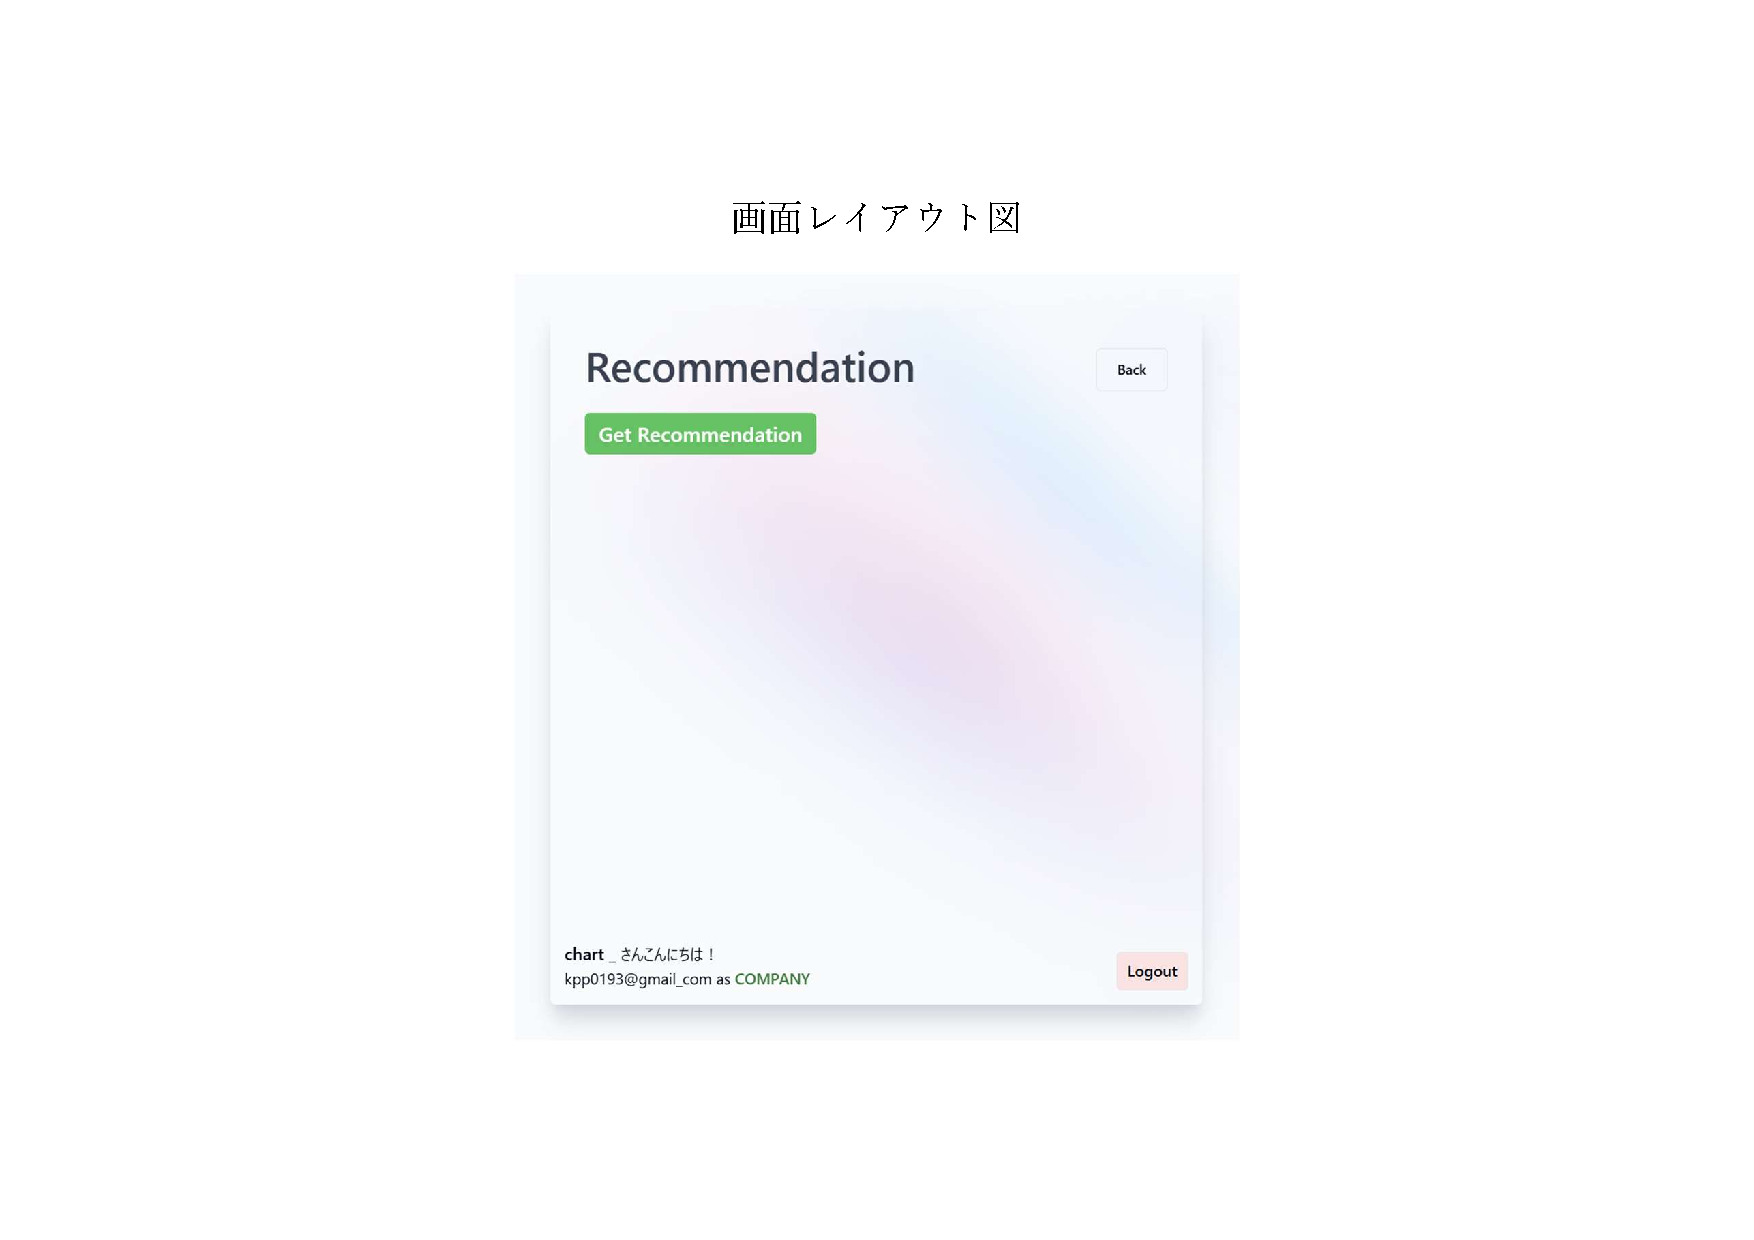
\includegraphics[trim=9cm 3.4cm 9cm 4.6cm, clip, width=\linewidth]{./img/recommend_company1.pdf}
        \caption{マッチング画面(企業)}
        \label{fig:recommend_company1}
    \end{subfigure}
    \caption{マッチング画面}
    \label{fig:recommend1}
\end{figure}
\vspace{-.5cm}

\begin{figure}[H]
    \centering
    \begin{subfigure}{0.49\textwidth}
        \centering
        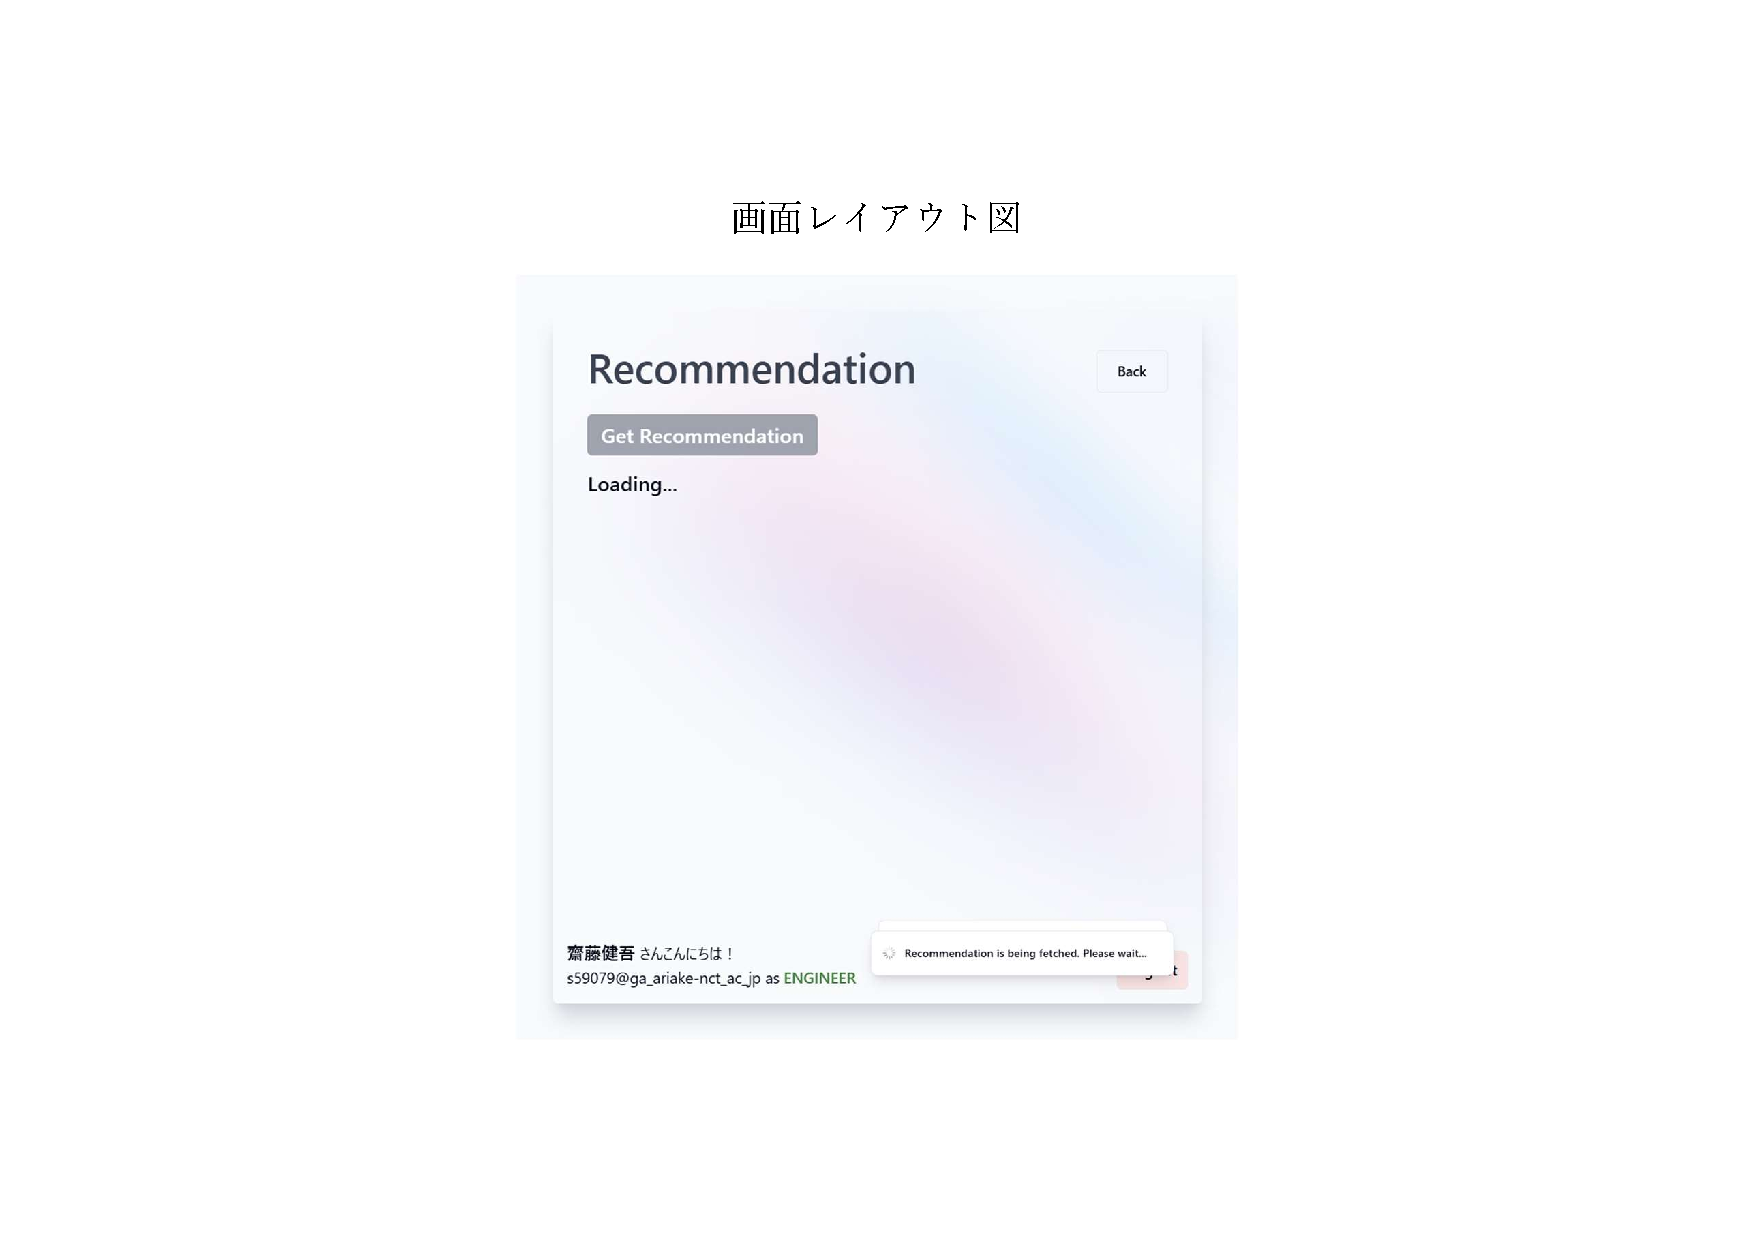
\includegraphics[trim=9cm 3.4cm 9cm 4.6cm, clip, width=\linewidth]{./img/recommend_engineer2.pdf}
        \caption{マッチング度計算中画面(エンジニア)}
        \label{fig:recommend_engineer2}
    \end{subfigure}
    \hfill
    \begin{subfigure}{0.49\textwidth}
        \centering
        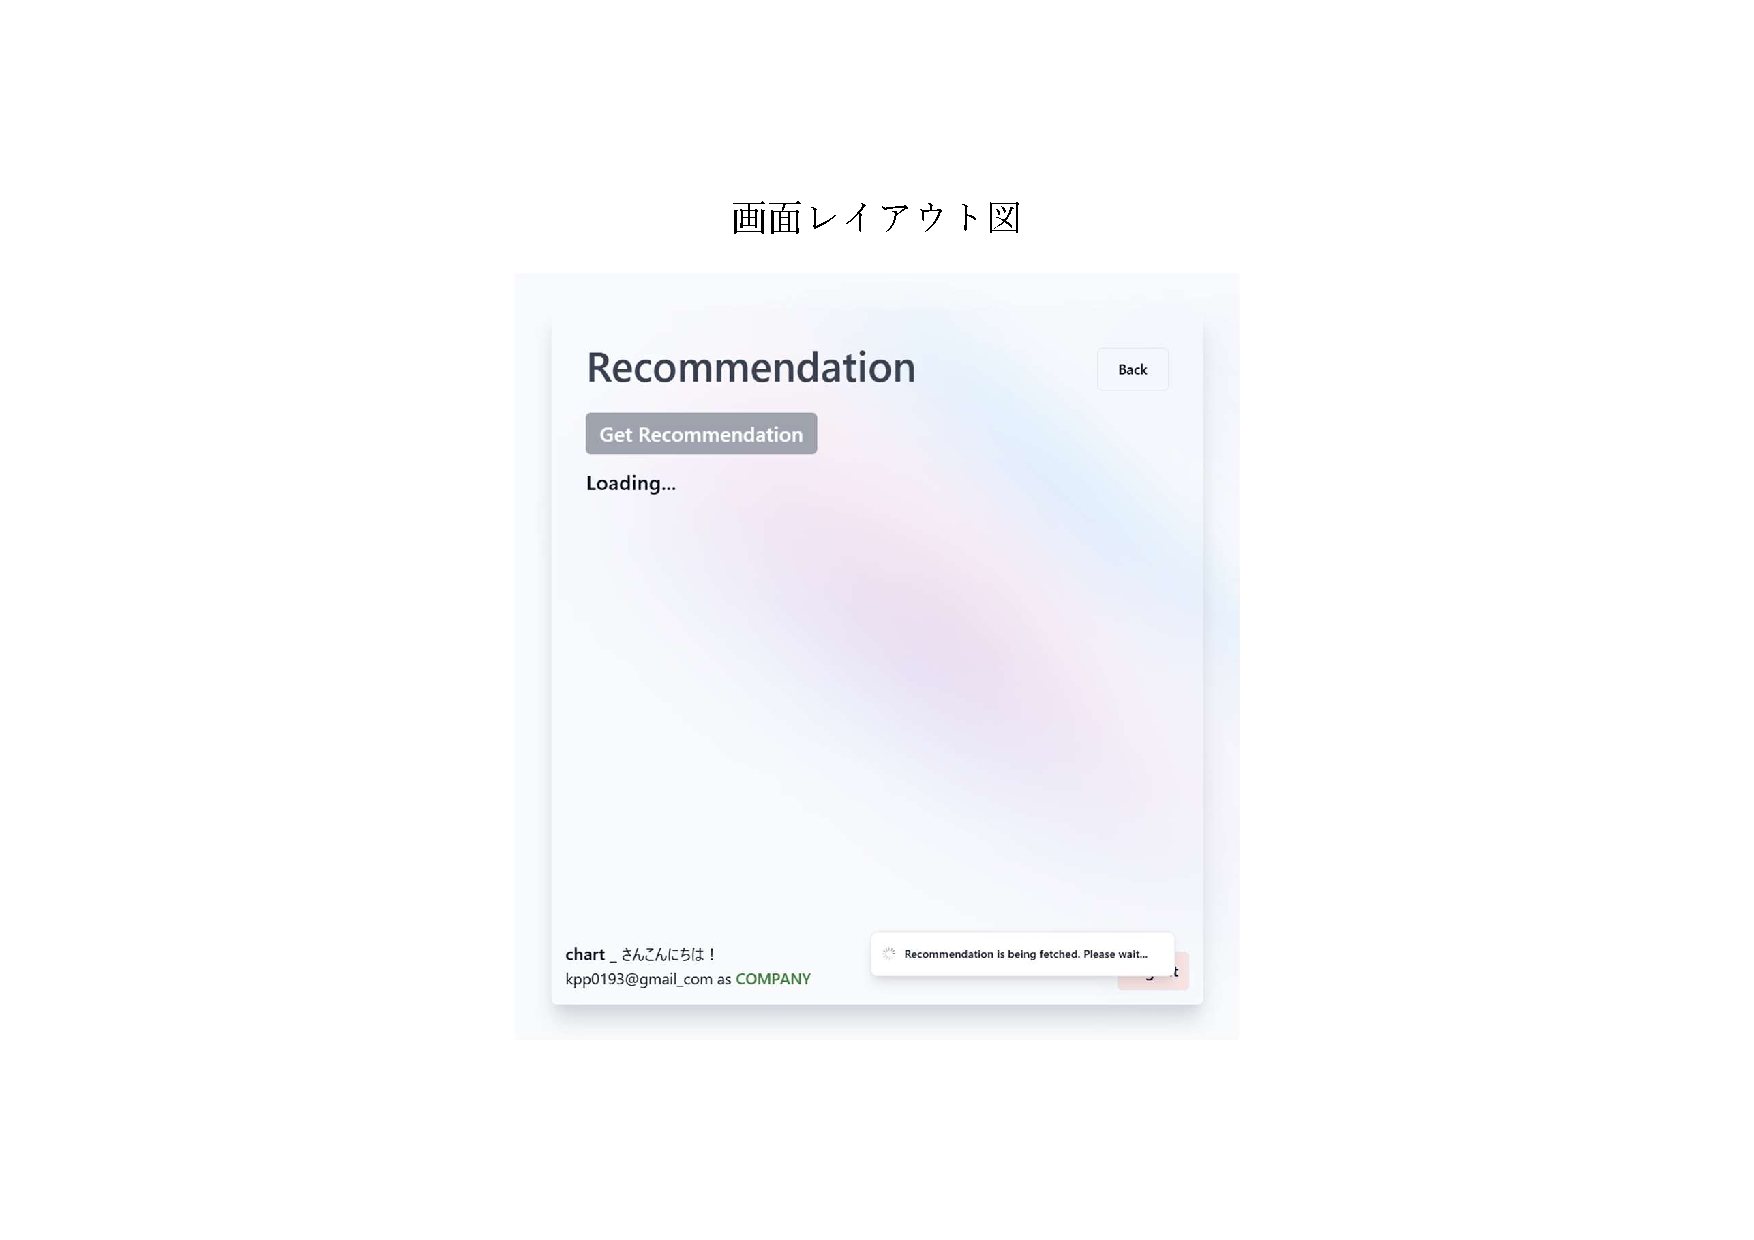
\includegraphics[trim=9cm 3.4cm 9cm 4.6cm, clip, width=\linewidth]{./img/recommend_company2.pdf}
        \caption{マッチング度計算中画面(企業)}
        \label{fig:recommend_company2}
    \end{subfigure}
    \caption{マッチング度計算中画面}
\end{figure}
\vspace{-.5cm}

\begin{figure}[H]
    \centering
    \begin{subfigure}{0.49\textwidth}
        \centering
        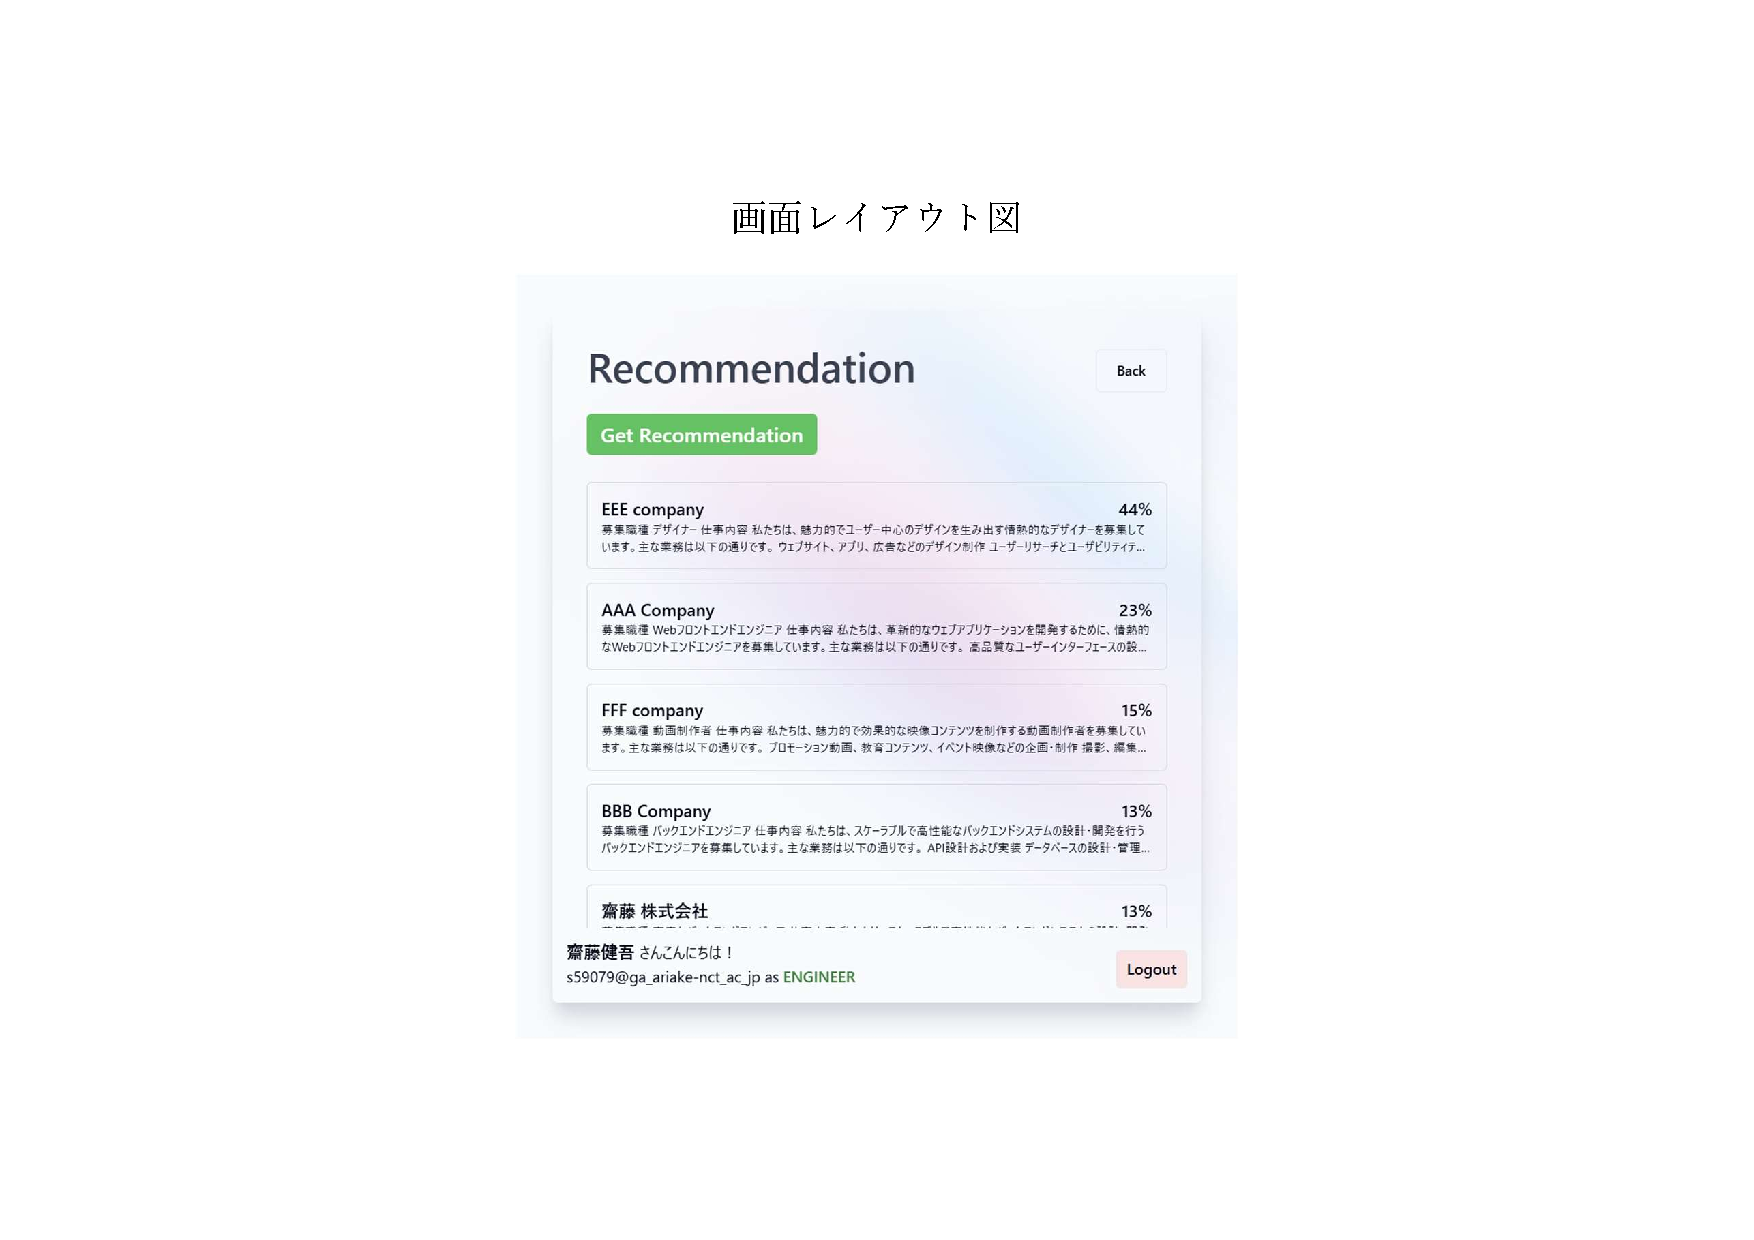
\includegraphics[trim=9cm 3.4cm 9cm 4.6cm, clip, width=\linewidth]{./img/recommend_engineer3.pdf}
        \caption{マッチング結果画面(エンジニア)}
        \label{fig:recommend_engineer3}
    \end{subfigure}
    \hfill
    \begin{subfigure}{0.49\textwidth}
        \centering
        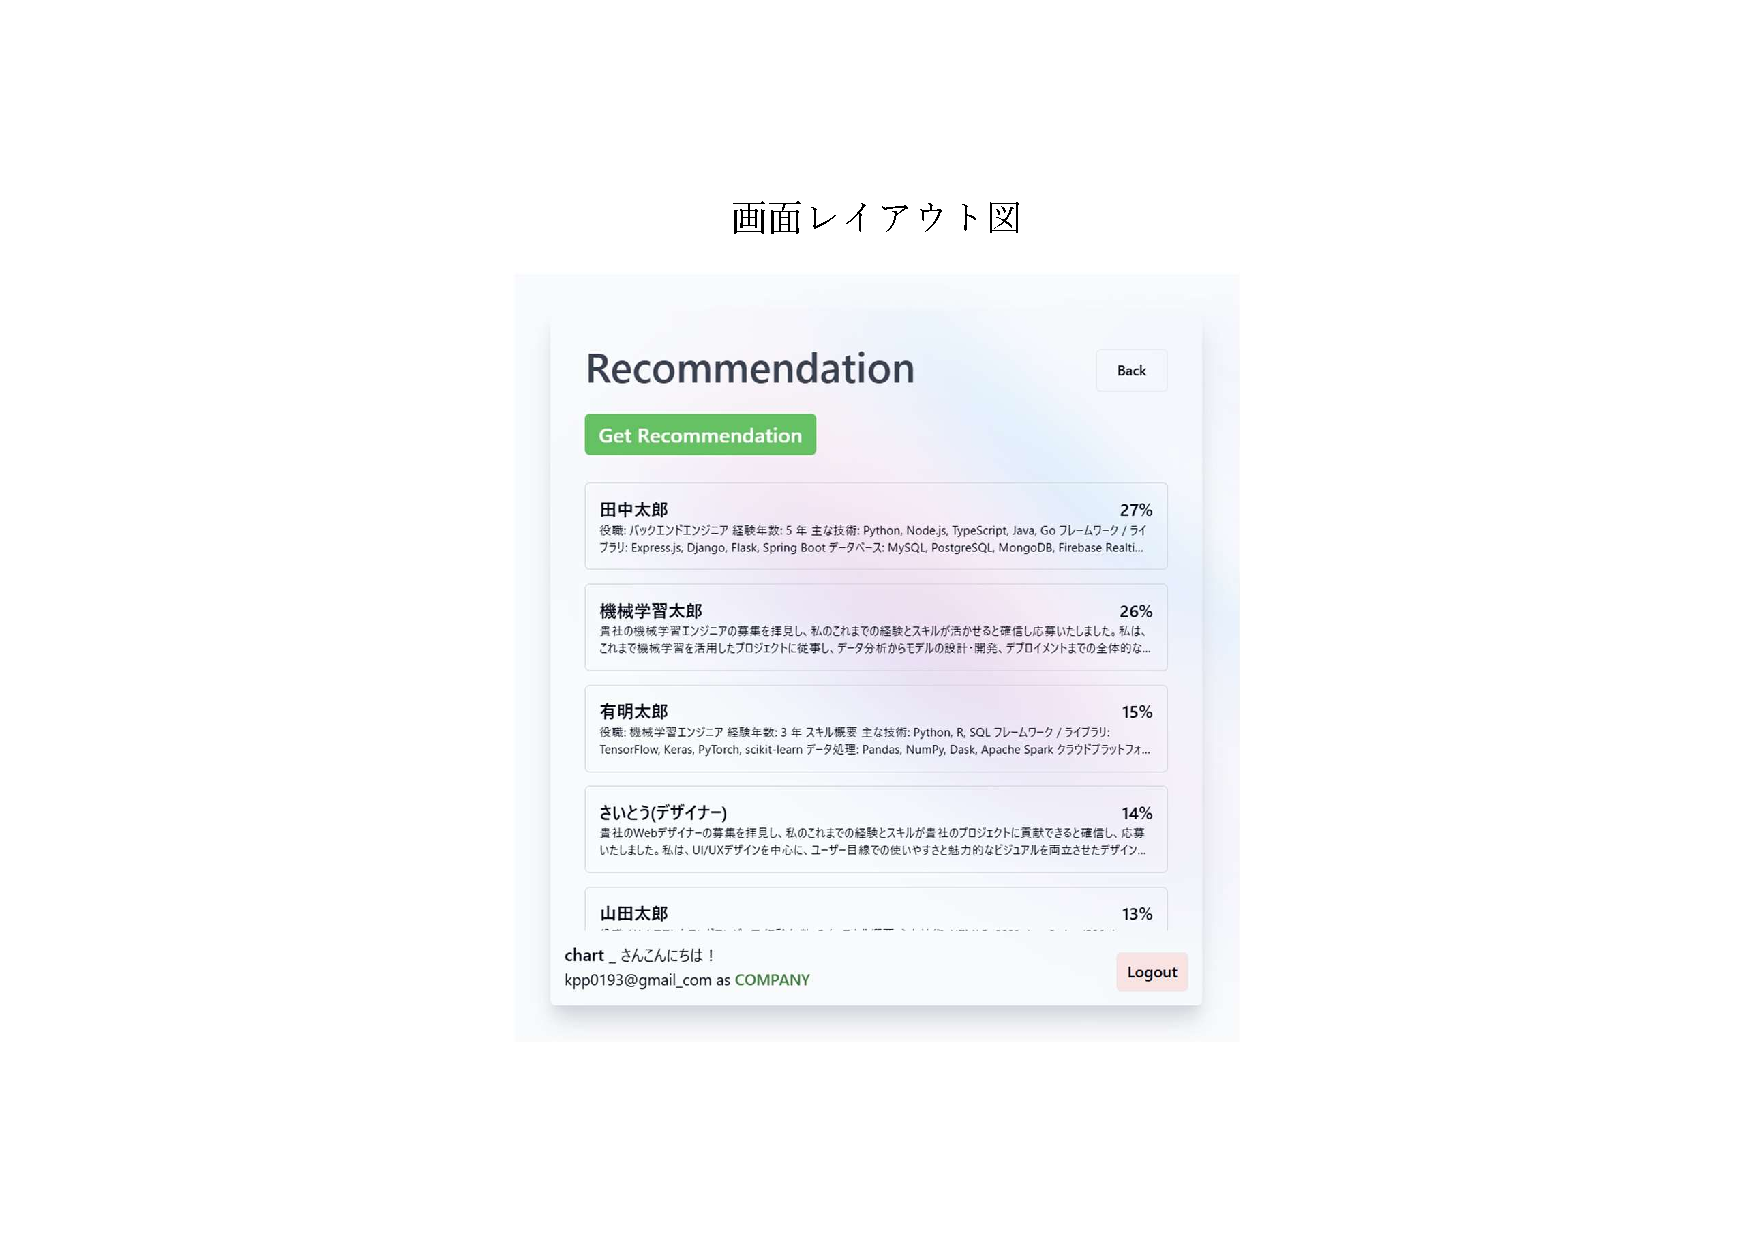
\includegraphics[trim=9cm 3.4cm 9cm 4.6cm, clip, width=\linewidth]{./img/recommend_company3.pdf}
        \caption{マッチング結果画面(企業)}
        \label{fig:recommend_company3}
    \end{subfigure}
    \caption{マッチング結果画面}
    \label{fig:recommend3}
\end{figure}
\vspace{-.5cm}

図\ref{fig:recommend_engineer1}は、エンジニアがマッチング画面を表示した際の画面を示しており、
図\ref{fig:recommend_company1}は、企業がマッチング画面を表示した際の画面を示している。\\
\indent Get Recommendation ボタンを押すと、
図\ref{fig:recommend_engineer2}, 図\ref{fig:recommend_company2}のように、マッチング度を計算中の画面に遷移し、
その間は Loading... と表示され、ボタンは押せなくなる。\\
\indent 図\ref{fig:recommend_engineer3}, 図\ref{fig:recommend_company3}は、マッチング結果画面を示しており、
エンジニアと企業の双方が、自身のアカウントに登録されている情報をもとに、
マッチング度を計算し、表示する画面である。\\
\indent より具体的には、自身のアカウントから投稿された1つの情報と、
異なるロールのアカウントから投稿された多数の情報を Tf-idf によりベクトル化し、
Cosine類似度を計算、ソートすることで、マッチング度を算出する。\\
\indent ゆえに、降順で表示される情報は、マッチング度が高い順になっており、
各情報の右側に表示されている値(%)は、Cosine類似度を100倍したものになっている。\\
\indent また、図\ref{fig:recommend3}は、
図\ref{fig:form_engineer}, 図\ref{fig:form_company} 
で投稿された情報に対する結果を示しており、このような出力が期待される。

% 参考文献
\begin{thebibliography}{9}
    \bibitem{nextjs} Next.js Documentation $\langle$\url{https://nextjs.org/docs}$\rangle$
    \bibitem{firebase} Firebase Documentation $\langle$\url{https://firebase.google.com/docs?hl=ja}$\rangle$
    % https://qiita.com/k-sukesakuma/items/4b56b9e81c1788d38440 「【Next.js】App Router × NextAuth.jsでGoogleログイン機能を実装したい 」
    \bibitem{nextauth} [Next.js] App Router × NextAuth.jsでGoogleログイン機能を実装したい $\langle$\url{https://qiita.com/k-sukesakuma/items/4b56b9e81c1788d38440}$\rangle$
    % はじめに: 最初の関数の記述、テスト、デプロイ - Firebase https://firebase.google.com/docs/functions/get-started?hl=ja
    \bibitem{firebase_function} はじめに: 最初の関数の記述、テスト、デプロイ - Firebase $\langle$\url{https://firebase.google.com/docs/functions/get-started?hl=ja}$\rangle$
    % https://dev.classmethod.jp/articles/firebase-functions-python/ Cloud Functions for FirebaseをPythonで使ってみた
    \bibitem{firebase_function_python} Cloud Functions for FirebaseをPythonで使ってみた $\langle$\url{https://dev.classmethod.jp/articles/firebase-functions-python/}$\rangle$
    % https://qiita.com/sai-san/items/24dbee74c5744033c330 [python] Firebase Realtime Databaseのはじめ方
    \bibitem{firebase_realtime} [python] Firebase Realtime Databaseのはじめ方 $\langle$\url{https://qiita.com/sai-san/items/24dbee74c5744033c330}$\rangle$
\end{thebibliography}

\end{document}
